\documentclass{report}
\usepackage[margin=2cm, bottom=1.5cm]{geometry}
\usepackage{type1cm}
\usepackage{amssymb}
\usepackage[fleqn]{amsmath}
\usepackage{tikz}
\usepackage{multicol}
\usepackage{makecell}
\usepackage{tabularx}
\usepackage[shortlabels]{enumitem}
\setlength{\columnsep}{1pt}
\setlist[enumerate]{nosep}

\makeatletter
\newenvironment{myalign*}{\ifvmode\else\hfil\null\linebreak\fi
  \hspace*{-\leftmargin}\minipage\textwidth
  \setlength{\abovedisplayskip}{0pt}%
  \setlength{\abovedisplayshortskip}{\abovedisplayskip}%
  \start@align\@ne\st@rredtrue\m@ne}%
{\endalign\endminipage\linebreak}

\usepackage{xeCJK}
\setCJKmainfont{Noto Sans TC}

\begin{document}
\title{%
	\fontsize{40}{60}\selectfont
	SCAF  \\ % 
	\vspace*{2cm}%
	\fontsize{24}{30}\selectfont
	設計文件
}

\author{
	\fontsize{18}{28}\selectfont
	\begin{tabularx}{0.9\textwidth}{
		|p{\dimexpr.25\linewidth-6\tabcolsep-2\arrayrulewidth}%
		|p{\dimexpr.75\linewidth-6\tabcolsep-2\arrayrulewidth}|%
		}
		\hline
		\centering 專案名稱 & SCAF 開發輔助工具                                       \\
		\hline
		\centering 撰寫日期 & 2022 / 11 / 21                                                \\
		\hline
		\centering 發展者    & 簡蔚驊 \! 鄧暐宣 \! 余威霆 \! 林佳何 \! 唐劭賢 \\
		\hline
	\end{tabularx}
}
\date{}
\usetikzlibrary{automata, positioning, arrows}
\maketitle
\tikzset{every state, accepting/.style={double distance=2pt}}

\fontsize{12}{18}\selectfont

\section*{1. 系統模型與架構(System Model/System Architecture)}

% \begin{obeylines}
% 	\parindent=0pt
% 	描述系統之架構。可用C4 model的Container diagram + Component diagram、UML之Component diagram或單純的Block diagram (方塊圖)表達此系統包含的模組,以及與模組之間的關係。
% 	架構圖應與SRS一致,但可特別強調介面(Interface)與實際佈署之環境。
% 	放C4所有的圖片
% 	鄧
% \end{obeylines}

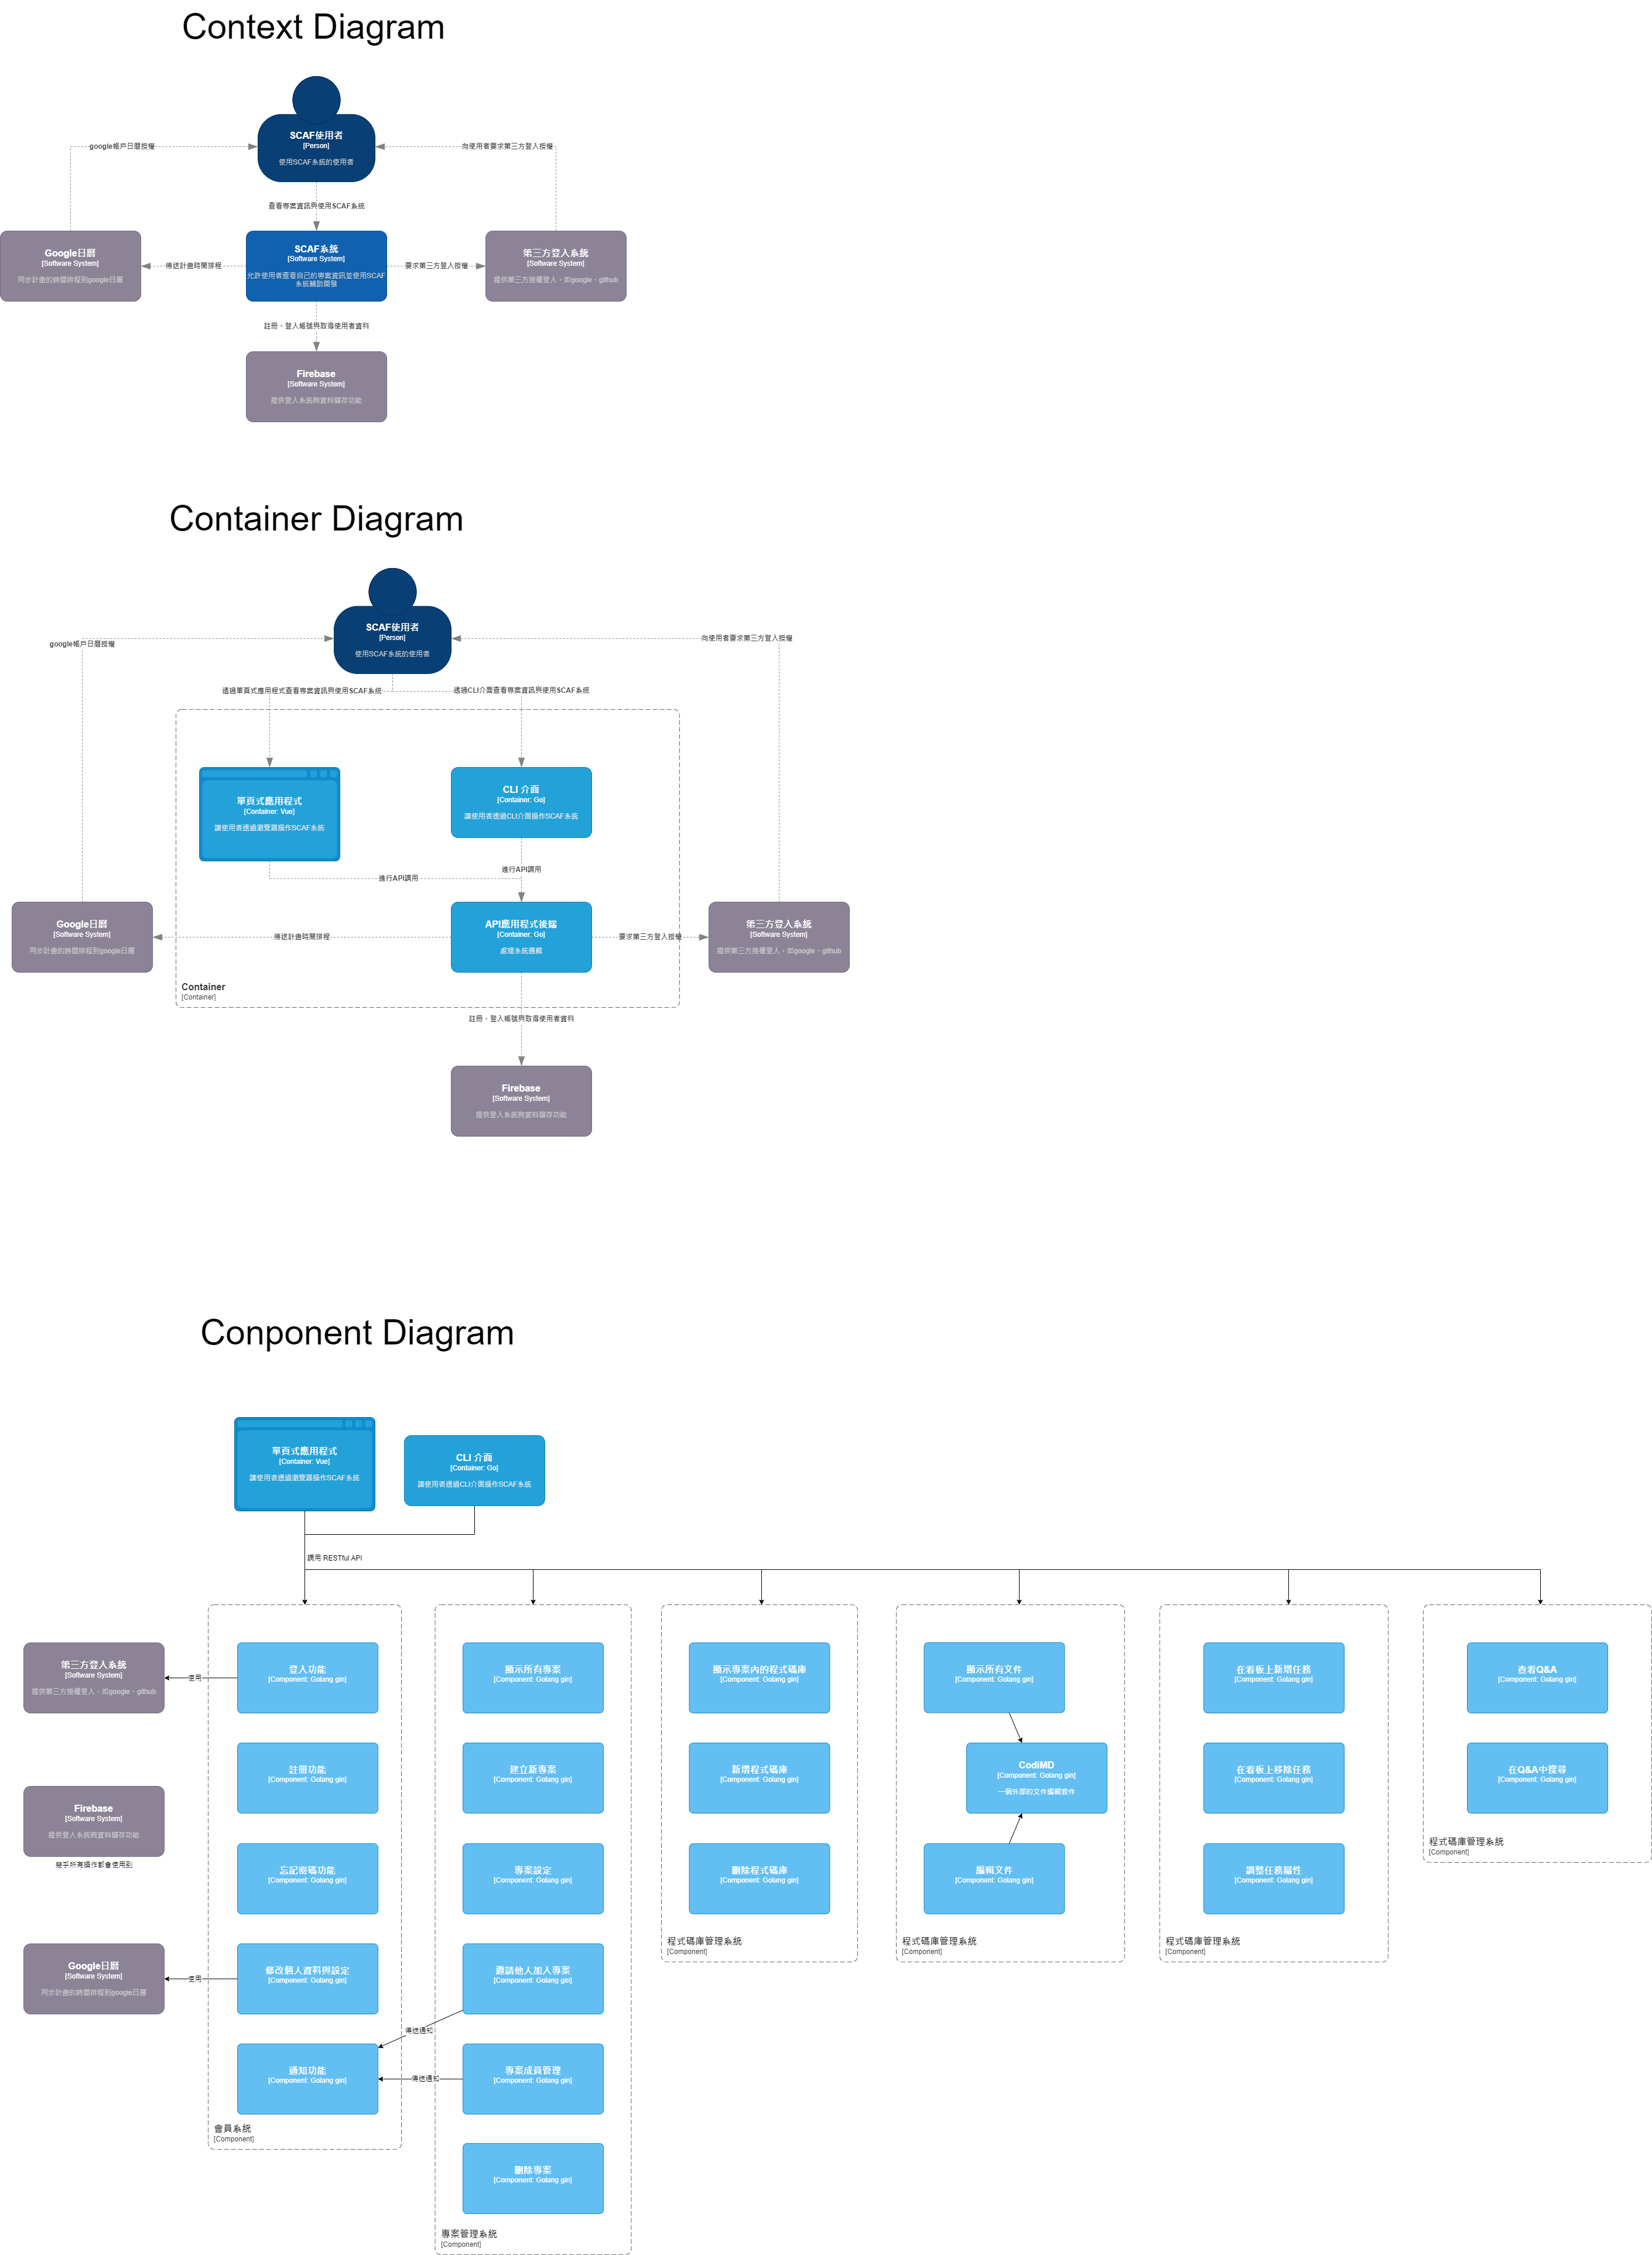
\includegraphics[width=\textwidth]{assets/SCAFC4.png}

\section*{2. 介面需求與設計(Interface Requirement and Design)}

% \newcolumntype{R}{>{\raggedleft}X}
\newcolumntype{R}{X}
\newcolumntype{T}{>{\hsize=\dimexpr2\hsize+2\tabcolsep+\arrayrulewidth\relax}X}
\newcolumntype{F}{>{\hsize=\dimexpr4\hsize+4\tabcolsep+\arrayrulewidth\relax}X}

\subsection*{2.1 會員子系統}

\subsubsection*{2.1.1 前端介面}

\begin{tabularx}{\textwidth}{|l|R|R|R|}
	\hline
	介面編號 & 介面名稱 & 介面提供者           & 介面使用者 \\ \hline
	AMM-EI-01    & 登入帳號 & Account Management Module &  Anyone           \\ \hline
	連結方式 & \multicolumn{2}{|c|}{輸入資料} & 輸出資料 \\ \hline
	& \multicolumn{2}{|T|}{email, password} & 登入成功後跳轉頁面 \\ \hline
	\multicolumn{4}{|c|}{對應介面之要求} \\ \hline
	\multicolumn{4}{|F|}{
	接收email及password,交由firebase驗證。驗證成功後,回傳token到前端。} \\ \hline
\end{tabularx}

\subsubsection*{}
\begin{tabularx}{\textwidth}{|l|R|R|R|}
	\hline
	介面編號 & 介面名稱 & 介面提供者           & 介面使用者 \\ \hline
	AMM-EI-02    & 註冊帳號 & Account Management Module & Anyone             \\ \hline
	連結方式 & \multicolumn{2}{|c|}{輸入資料} & 輸出資料 \\ \hline
	& \multicolumn{2}{|T|}{email, password} & 註冊成功後跳轉頁面 \\ \hline
	\multicolumn{4}{|c|}{對應介面之要求} \\ \hline
	\multicolumn{4}{|F|}{
	接收email及password,交由firebase註冊。} \\ \hline
\end{tabularx}

\subsubsection*{}
\begin{tabularx}{\textwidth}{|l|R|R|R|}
	\hline
	介面編號 & 介面名稱 & 介面提供者           & 介面使用者 \\ \hline
	AMM-EI-03    & 忘記密碼 & Account Management Module & Anyone          \\ \hline
	連結方式 & \multicolumn{2}{|c|}{輸入資料} & 輸出資料 \\ \hline
	& \multicolumn{2}{|T|}{email} & 驗證完後跳回登入頁 \\ \hline
	\multicolumn{4}{|c|}{對應介面之要求} \\ \hline
	\multicolumn{4}{|F|}{
	接收email,交由firebase驗證,並由firebase寄送驗證信到使用者上。} \\ \hline
\end{tabularx}

\subsubsection*{}
\begin{tabularx}{\textwidth}{|l|R|R|R|}
	\hline
	介面編號 & 介面名稱       & 介面提供者           & 介面使用者 \\ \hline
	AMM-EI-04    & 修改個人資料 & Account Management Module & Member            \\ \hline
	連結方式 & \multicolumn{2}{|c|}{輸入資料} & 輸出資料 \\ \hline
	& \multicolumn{2}{|T|}{avatar, nickname, bio} & 顯示新的個人資料 \\ \hline
	\multicolumn{4}{|c|}{對應介面之要求} \\ \hline
	\multicolumn{4}{|F|}{
	接收收avatar、nickname、bio,將資料交給firebase儲存。} \\ \hline
\end{tabularx}

\subsubsection*{}
\begin{tabularx}{\textwidth}{|l|R|R|R|}
	\hline
	介面編號 & 介面名稱 & 介面提供者           & 介面使用者 \\ \hline
	AMM-EI-05    & 修改密碼 & Account Management Module & Member            \\ \hline
	連結方式 & \multicolumn{2}{|c|}{輸入資料} & 輸出資料 \\ \hline
	& \multicolumn{2}{|T|}{old password, new password} & 跳到登入畫面 \\ \hline
	\multicolumn{4}{|c|}{對應介面之要求} \\ \hline
	\multicolumn{4}{|F|}{
	接收old password、new password,old password與firebase驗證過後,將new password交給firebase做更新。} \\ \hline
\end{tabularx}

\subsubsection*{}
\begin{tabularx}{\textwidth}{|l|R|R|R|}
	\hline
	介面編號 & 介面名稱        & 介面提供者           & 介面使用者 \\ \hline
	AMM-EI-06    & Google 日曆授權 & Account Management Module & SCAF系統            \\ \hline
	連結方式 & \multicolumn{2}{|c|}{輸入資料} & 輸出資料 \\ \hline
	& \multicolumn{2}{|T|}{} &  授權結果 \\ \hline
	\multicolumn{4}{|c|}{對應介面之要求} \\ \hline
	\multicolumn{4}{|F|}{
	透過Google日曆 API 管理授權} \\ \hline
\end{tabularx}

\subsubsection*{}
\begin{tabularx}{\textwidth}{|l|R|R|R|}
	\hline
	介面編號 & 介面名稱 & 介面提供者           & 介面使用者 \\ \hline
	AMM-EI-07    & 取得通知 & Account Management Module & Member            \\ \hline
	連結方式 & \multicolumn{2}{|c|}{輸入資料} & 輸出資料 \\ \hline
	& \multicolumn{2}{|T|}{} &  顯示通知訊息 \\ \hline
	\multicolumn{4}{|c|}{對應介面之要求} \\ \hline
	\multicolumn{4}{|F|}{
	系統上顯示傳給使用者的通知} \\ \hline
\end{tabularx}

\subsubsection*{2.1.2 後端介面}

\subsubsection*{}
\begin{tabularx}{\textwidth}{|l|R|R|R|}
	\hline
	介面編號 & 介面名稱 & 介面提供者           & 介面使用者 \\ \hline
	AMM-II-01    & /signin      & Account Management Module & Client端            \\ \hline
	連結方式 & \multicolumn{2}{|c|}{輸入資料} & 輸出資料 \\ \hline
	POST & \multicolumn{2}{|T|}{
	\makecell[l]{
	\{ \\
	"email": "Email (string)", \\
	"password": "Password (string)" \\
	\}      
	}
	} & 
	\makecell[X]{
	\{ \\
	"status": "Status (string, 200)", \\
	"message": "訊息 (string)" \\
	"JWT": "JWT token (string)" \\
	\}
	}
	\\ \hline
	\multicolumn{4}{|c|}{對應介面之要求} \\ \hline
	\multicolumn{4}{|F|}{
	將登入資訊傳給firebase進行資料驗證,接收回傳結果} \\ \hline
\end{tabularx}

\subsubsection*{}
\begin{tabularx}{\textwidth}{|l|R|R|R|}
	\hline
	介面編號 & 介面名稱 & 介面提供者           & 介面使用者 \\ \hline
	AMM-II-02    & /signup      & Account Management Module & Client端            \\ \hline
	連結方式 & \multicolumn{2}{|c|}{輸入資料} & 輸出資料 \\ \hline
	POST & \multicolumn{2}{|T|}{
	\makecell[l]{
	\{ \\
	"email": "Email (string)", \\
	"password": "Password (string)" \\
	\}      
	}
	} & 
	\makecell[X]{
	\{ \\
	"status": "Status (string, 200)", \\
	"message": "訊息 (string)" \\
	"JWT": "JWT token (string)" \\
	\}
	}
	\\ \hline
	\multicolumn{4}{|c|}{對應介面之要求} \\ \hline
	\multicolumn{4}{|F|}{
	將註冊資訊傳給firebase,驗證後加入資料庫} \\ \hline
\end{tabularx}

\subsubsection*{}
\begin{tabularx}{\textwidth}{|l|R|R|R|}
	\hline
	介面編號 & 介面名稱 & 介面提供者           & 介面使用者 \\ \hline
	AMM-II-03    & /forget      & Account Management Module & Client端            \\ \hline
	連結方式 & \multicolumn{2}{|c|}{輸入資料} & 輸出資料 \\ \hline
	POST & \multicolumn{2}{|T|}{
	\makecell[l]{
	\{ \\
	"email": "Email (string)", \\
	\}      
	}
	} & 
	\makecell[X]{
	\{ \\
	"status": "Status (string, 200)" \\
	"message": "訊息 (string)" \\
	\}
	}
	\\ \hline
	\multicolumn{4}{|c|}{對應介面之要求} \\ \hline
	\multicolumn{4}{|F|}{
	傳送email,交給firebase寄信重設密碼} \\ \hline
\end{tabularx}

\subsubsection*{}
\begin{tabularx}{\textwidth}{|l|R|R|R|}
	\hline
	介面編號 & 介面名稱 & 介面提供者           & 介面使用者 \\ \hline
	AMM-II-04    & /user      & Account Management Module & Client端            \\ \hline
	連結方式 & \multicolumn{2}{|c|}{輸入資料} & 輸出資料 \\ \hline
	PUT & \multicolumn{2}{|T|}{
	\makecell[l]{
	\{ \\
	"JWT": "JWT token (string, cookie)", \\
	"avatar": "Avatar (base64)", \\
	"nickname": "Nickname (string)", \\
	"bio": "bio (string)" \\
	\}      
	}
	} & 
	\makecell[X]{
	\{ \\
	"status": "Status (string, 200)" \\
	"message": "訊息 (string)" \\
	\}
	}
	\\ \hline
	\multicolumn{4}{|c|}{對應介面之要求} \\ \hline
	\multicolumn{4}{|F|}{
	將個人資訊傳給firebase,根據 JWT 找到帳戶進行儲存,回傳狀態} \\ \hline
\end{tabularx}

\subsubsection*{}
\begin{tabularx}{\textwidth}{|l|R|R|R|}
	\hline
	介面編號 & 介面名稱 & 介面提供者           & 介面使用者 \\ \hline
	AMM-II-05    & /user/*uid     & Account Management Module & Client端            \\ \hline
	連結方式 & \multicolumn{2}{|c|}{輸入資料} & 輸出資料 \\ \hline
	GET & \multicolumn{2}{|T|}{
	\makecell[l]{
	\{ \\
	"JWT": "JWT token (string, cookie)", \\
	\}      
	}
	} & 
	\makecell[X]{
	\{ \\
	"status": "Status (string, 200)", \\
	"message": "訊息 (string)" \\
	"avatar": "Avatar (base64)", \\
	"nickname": "Nickname (string)", \\
	"bio": "bio (string)" \\
	\}
	}
	\\ \hline
	\multicolumn{4}{|c|}{對應介面之要求} \\ \hline
	\multicolumn{4}{|F|}{
	由 uid 從firebase獲得使用者資料,若 uid 為空則為代表自己。} \\ \hline
\end{tabularx}

\subsubsection*{}
\begin{tabularx}{\textwidth}{|l|R|R|R|}
	\hline
	介面編號 & 介面名稱  & 介面提供者           & 介面使用者 \\ \hline
	AMM-II-06    & /user/reset & Account Management Module & Client端            \\ \hline
	連結方式 & \multicolumn{2}{|c|}{輸入資料} & 輸出資料 \\ \hline
	POST & \multicolumn{2}{|T|}{
	\makecell[l]{
	\{ \\
	"JWT": "JWT token (string, cookie)", \\
	"oldPassword": "Password (string)", \\
	"newPassword": "Password (string)", \\
	\}      
	}
	} & 
	\makecell[X]{
	\{ \\
	"status": "Status (string, 200)", \\
	"message": "訊息 (string)" \\
	\}
	}
	\\ \hline
	\multicolumn{4}{|c|}{對應介面之要求} \\ \hline
	\multicolumn{4}{|F|}{
	Firebase確認oldPassword後,更新Firebase中password資訊。} \\ \hline
\end{tabularx}

\subsubsection*{}
\begin{tabularx}{\textwidth}{|l|R|R|R|}
	\hline
	介面編號 & 介面名稱     & 介面提供者           & 介面使用者 \\ \hline
	AMM-II-07    & /user/calendar & Account Management Module & Client端            \\ \hline
	連結方式 & \multicolumn{2}{|c|}{輸入資料} & 輸出資料 \\ \hline
	POST & \multicolumn{2}{|T|}{
	\makecell[l]{
	\{ \\
	"JWT": "JWT token (string, cookie)", \\
	\}      
	}
	} & 
	\makecell[X]{
	\{ \\
	"status": "Status (string, 200)", \\
	"message": "訊息 (string)" \\
	\}
	}
	\\ \hline
	\multicolumn{4}{|c|}{對應介面之要求} \\ \hline
	\multicolumn{4}{|F|}{
	透過Google日曆 API 管理授權} \\ \hline
\end{tabularx}

\subsubsection*{}
\begin{tabularx}{\textwidth}{|l|R|R|R|}
	\hline
	介面編號 & 介面名稱 & 介面提供者           & 介面使用者 \\ \hline
	AMM-II-08    & /notify      & Account Management Module & Client端            \\ \hline
	連結方式 & \multicolumn{2}{|c|}{輸入資料} & 輸出資料 \\ \hline
	GET & \multicolumn{2}{|T|}{
	\makecell[l]{
	\{ \\
	"JWT": "JWT token (string, cookie)", \\
	\}      
	}
	} & 
	\makecell[X]{
	\{ \\
	"status": "Status (string, 200)", \\
	"message": "訊息 (string)" \\
	\}
	}
	\\ \hline
	\multicolumn{4}{|c|}{對應介面之要求} \\ \hline
	\multicolumn{4}{|F|}{
	系統上顯示傳給使用者的通知} \\ \hline
\end{tabularx}

\subsection*{2.2 專案管理子系統}

\subsubsection*{2.2.1 前端介面}

\subsubsection*{}
\begin{tabularx}{\textwidth}{|l|R|R|R|}
	\hline
	介面編號 & 介面名稱       & 介面提供者           & 介面使用者 \\ \hline
	PMM-EI-01    & 列出所有專案 & Project Management Module & Member            \\ \hline
	連結方式 & \multicolumn{2}{|c|}{輸入資料} & 輸出資料 \\ \hline
	& \multicolumn{2}{|T|}{
	\makecell[l]{}
	} & 
	\makecell[X]{
	列出所有專案的資料
	}
	\\ \hline
	\multicolumn{4}{|c|}{對應介面之要求} \\ \hline
	\multicolumn{4}{|F|}{
	根據登入的帳戶,回傳對應的專案資訊} \\ \hline
\end{tabularx}

\subsubsection*{}
\begin{tabularx}{\textwidth}{|l|R|R|R|}
	\hline
	介面編號 & 介面名稱    & 介面提供者           & 介面使用者 \\ \hline
	PMM-EI-02    & 建立新專案 & Project Management Module & Member             \\ \hline
	連結方式 & \multicolumn{2}{|c|}{輸入資料} & 輸出資料 \\ \hline
	& \multicolumn{2}{|T|}{
	\makecell[l]{
	Project Name, Development Mode
	}
	} & 
	\makecell[X]{
	新增完專案後,跳到專案畫面。
	}
	\\ \hline
	\multicolumn{4}{|c|}{對應介面之要求} \\ \hline
	\multicolumn{4}{|F|}{
	接收Project Name、Development mode,將資料丟給firebase儲存,並跳轉頁面} \\ \hline
\end{tabularx}

\subsubsection*{}
\begin{tabularx}{\textwidth}{|l|R|R|R|}
	\hline
	介面編號 & 介面名稱  & 介面提供者           & 介面使用者 \\ \hline
	PMM-EI-03    & 新建 Readme & Project Management Module & Member              \\ \hline
	連結方式 & \multicolumn{2}{|c|}{輸入資料} & 輸出資料 \\ \hline
	& \multicolumn{2}{|T|}{
	\makecell[l]{
	% 
	}
	} & 
	\makecell[X]{
	建立 Readme 檔案
	}
	\\ \hline
	\multicolumn{4}{|c|}{對應介面之要求} \\ \hline
	\multicolumn{4}{|F|}{
	當有選則要建立Readme時,會自動建立Readme} \\ \hline
\end{tabularx}

\subsubsection*{}
\begin{tabularx}{\textwidth}{|l|R|R|R|}
	\hline
	介面編號 & 介面名稱       & 介面提供者           & 介面使用者 \\ \hline
	PMM-EI-04    & 專案設定修改 & Project Management Module & Project owner            \\ \hline
	連結方式 & \multicolumn{2}{|c|}{輸入資料} & 輸出資料 \\ \hline
	& \multicolumn{2}{|T|}{
	\makecell[l]{
	Project Name, Development Mode
	}
	} & 
	\makecell[X]{
	修改完專案設定後,跳到專案畫面。
	}
	\\ \hline
	\multicolumn{4}{|c|}{對應介面之要求} \\ \hline
	\multicolumn{4}{|F|}{
	接收Project Name、Development Mode,交給firebase,跳轉頁面} \\ \hline
\end{tabularx}

\subsubsection*{}
\begin{tabularx}{\textwidth}{|l|R|R|R|}
	\hline
	介面編號 & 介面名稱       & 介面提供者           & 介面使用者 \\ \hline
	PMM-EI-05    & 邀請加入專案 & Project Management Module & Project owner            \\ \hline
	連結方式 & \multicolumn{2}{|c|}{輸入資料} & 輸出資料 \\ \hline
	& \multicolumn{2}{|T|}{
	\makecell[l]{
	User Mail
	}
	} & 
	\makecell[X]{
	邀請成功後,跳出成功邀請通知。
	}
	\\ \hline
	\multicolumn{4}{|c|}{對應介面之要求} \\ \hline
	\multicolumn{4}{|F|}{
	透過Firebase寄送訊息給User Mail} \\ \hline
\end{tabularx}

\subsubsection*{}
\begin{tabularx}{\textwidth}{|l|R|R|R|}
	\hline
	介面編號 & 介面名稱 & 介面提供者           & 介面使用者 \\ \hline
	PMM-EI-06    & 移除成員 & Project Management Module & Project owner            \\ \hline
	連結方式 & \multicolumn{2}{|c|}{輸入資料} & 輸出資料 \\ \hline
	& \multicolumn{2}{|T|}{
	\makecell[l]{
	User Mail
	}
	} & 
	\makecell[X]{
	移除成功後,跳出成功移除通知。
	}
	\\ \hline
	\multicolumn{4}{|c|}{對應介面之要求} \\ \hline
	\multicolumn{4}{|F|}{
	接收User Mail並交給Firebase,Firebase移除專案中成員。} \\ \hline
\end{tabularx}

\subsubsection*{}
\begin{tabularx}{\textwidth}{|l|R|R|R|}
	\hline
	介面編號 & 介面名稱 & 介面提供者           & 介面使用者 \\ \hline
	PMM-EI-07    & 刪除專案 & Project Management Module & Project owner            \\ \hline
	連結方式 & \multicolumn{2}{|c|}{輸入資料} & 輸出資料 \\ \hline
	& \multicolumn{2}{|T|}{
	\makecell[l]{
	%  
	}
	} & 
	\makecell[X]{
	刪除完專案,跳回到專案列表。
	}
	\\ \hline
	\multicolumn{4}{|c|}{對應介面之要求} \\ \hline
	\multicolumn{4}{|F|}{
	刪除使用者點擊的專案,並跳回專案列表。} \\ \hline
\end{tabularx}

\subsubsection*{2.2.2 後端介面}

註: 前綴 /project 前包含 /user/:uid

\subsubsection*{}
\begin{tabularx}{\textwidth}{|l|R|R|R|}
	\hline
	介面編號 & 介面名稱 & 介面提供者           & 介面使用者 \\ \hline
	PMM-II-01    & /projects    & Project Management Module & Client端            \\ \hline
	連結方式 & \multicolumn{2}{|c|}{輸入資料} & 輸出資料 \\ \hline
	GET & \multicolumn{2}{|T|}{
	\makecell[l]{
	\{ \\
	"JWT": "JWT token (string, cookie)"  \\
	\} 
	}
	} & 
	\makecell[X]{
	\{ \\
	"status" : "Status (string)", \\
	"message": "訊息 (string)" \\
	"projects": "專案列表 (Array<{string, projectname}>)" \\
	\}
	}
	\\ \hline
	\multicolumn{4}{|c|}{對應介面之要求} \\ \hline
	\multicolumn{4}{|F|}{
	根據登入的帳戶,取得firebase回傳的專案列表。若 JWT 代表的 user token 與 uid 不符,則回傳錯誤訊息。} \\ \hline
\end{tabularx}

\subsubsection*{}
\begin{tabularx}{\textwidth}{|l|R|R|R|}
	\hline
	介面編號 & 介面名稱 & 介面提供者           & 介面使用者 \\ \hline
	PMM-II-02    & /project     & Project Management Module & Client端            \\ \hline
	連結方式 & \multicolumn{2}{|c|}{輸入資料} & 輸出資料 \\ \hline
	POST & \multicolumn{2}{|T|}{
	\makecell[l]{
	\{ \\
	"JWT": "JWT token (string, cookie)"  \\
	"name": "project name (string)", \\
	"devMode": "development mode (string)", \\
	"devTools": "development tools (Array<string>)", \\
	\}
	}
	} & 
	\makecell[X]{
	\{ \\
	"status": "Status (string)", \\
	"message": "訊息 (string)" \\
	"name" : "專案名稱 (string)", \\
	\}
	}
	\\ \hline
	\multicolumn{4}{|c|}{對應介面之要求} \\ \hline
	\multicolumn{4}{|F|}{
	傳projectname、developmentmode給firebase,firebase新增專案資訊。
	projectname 對於每個使用者都是唯一的。
	} \\ \hline
\end{tabularx}

\subsubsection*{}
\begin{tabularx}{\textwidth}{|l|R|R|R|}
	\hline
	介面編號 & 介面名稱    & 介面提供者           & 介面使用者 \\ \hline
	PMM-II-03    & /project/:pn/readme & Project Management Module & Client端            \\ \hline
	連結方式 & \multicolumn{2}{|c|}{輸入資料} & 輸出資料 \\ \hline
	POST & \multicolumn{2}{|T|}{
	\makecell[l]{
	\{ \\
	"JWT": "JWT token (string, cookie)",  \\  
	\}
	}
	} & 
	\makecell[X]{
	\{ \\
	"status": "Status (string)", \\
	"message": "訊息 (string)" \\
	\}
	}
	\\ \hline
	\multicolumn{4}{|c|}{對應介面之要求} \\ \hline
	\multicolumn{4}{|F|}{
	若有選擇加入readme,則在firebase中建立readme資訊
	} \\ \hline
\end{tabularx}

\subsubsection*{}
\begin{tabularx}{\textwidth}{|l|R|R|R|}
	\hline
	介面編號 & 介面名稱 & 介面提供者           & 介面使用者 \\ \hline
	PMM-II-04    & /project/:pn/  & Project Management Module & Client端            \\ \hline
	連結方式 & \multicolumn{2}{|c|}{輸入資料} & 輸出資料 \\ \hline
	PUT & \multicolumn{2}{|T|}{
	\makecell[l]{
	\{ \\
	"JWT": "JWT token (string, cookie)"  \\
	"name": "project name (string)", \\
	"devMode": "development mode (string)", \\
	"devTools": "development tools (Array<string>)", \\
	\}
	}
	} & 
	\makecell[X]{
	\{ \\
	"status": "Status (string)", \\
	"message": "訊息 (string)" \\
	\}
	}
	\\ \hline
	\multicolumn{4}{|c|}{對應介面之要求} \\ \hline
	\multicolumn{4}{|F|}{
	傳project name、development mode給firebase,firebase更新專案資訊。
	projectname 對於每個使用者都是唯一的。

	} \\ \hline
\end{tabularx}

\subsubsection*{}
\begin{tabularx}{\textwidth}{|l|R|R|R|}
	\hline
	介面編號 & 介面名稱    & 介面提供者           & 介面使用者 \\ \hline
	PMM-II-05    & /project/:pn/member & Project Management Module & Client端            \\ \hline
	連結方式 & \multicolumn{2}{|c|}{輸入資料} & 輸出資料 \\ \hline
	GET & \multicolumn{2}{|T|}{
	\makecell[l]{
	\{ \\
	"JWT": "JWT token (string, cookie)",  \\  
	\}
	}
	} & 
	\makecell[X]{
	\{ \\
	"status": "Status (string)", \\
	"message": "訊息 (string)" \\
	\}
	}
	\\ \hline
	\multicolumn{4}{|c|}{對應介面之要求} \\ \hline
	\multicolumn{4}{|F|}{
	獲取專案成員列表
	} \\ \hline
\end{tabularx}

\subsubsection*{}
\begin{tabularx}{\textwidth}{|l|R|R|R|}
	\hline
	介面編號 & 介面名稱    & 介面提供者           & 介面使用者 \\ \hline
	PMM-II-06    & \makecell[X]{/project/:pn/member\\/:uid} & Project Management Module & Client端            \\ \hline
	連結方式 & \multicolumn{2}{|c|}{輸入資料} & 輸出資料 \\ \hline
	POST & \multicolumn{2}{|T|}{
	\makecell[l]{
	\{ \\
	"JWT": "JWT token (string, cookie)",  \\  
	\}
	}
	} & 
	\makecell[X]{
	\{ \\
	"status": "Status (string)", \\
	"message": "訊息 (string)" \\
	\}
	}
	\\ \hline
	\multicolumn{4}{|c|}{對應介面之要求} \\ \hline
	\multicolumn{4}{|F|}{
	傳mail給firebase,firebase發送邀請決定。,是否讓firebase新增專案成員資訊。 
	} \\ \hline
\end{tabularx}

\subsubsection*{}
\begin{tabularx}{\textwidth}{|l|R|R|R|}
	\hline
	介面編號 & 介面名稱    & 介面提供者           & 介面使用者 \\ \hline
	PMM-II-07    & \makecell[X]{/project/:pn/member\\/:uid} & Project Management Module & Client端            \\ \hline
	連結方式 & \multicolumn{2}{|c|}{輸入資料} & 輸出資料 \\ \hline
	DELETE & \multicolumn{2}{|T|}{
	\makecell[l]{
	\{ \\
	"JWT": "JWT token (string, cookie)",  \\  
	\}
	}
	} & 
	\makecell[X]{
	\{ \\
	"status": "Status (string)", \\
	"message": "訊息 (string)" \\
	\}
	}
	\\ \hline
	\multicolumn{4}{|c|}{對應介面之要求} \\ \hline
	\multicolumn{4}{|F|}{
	根據usermail,刪除firebase專案中成員資訊。
	} \\ \hline
\end{tabularx}

\subsubsection*{}
\begin{tabularx}{\textwidth}{|l|R|R|R|}
	\hline
	介面編號 & 介面名稱 & 介面提供者           & 介面使用者 \\ \hline
	PMM-II-03    & /project/:pn/     & Project Management Module & Client端            \\ \hline
	連結方式 & \multicolumn{2}{|c|}{輸入資料} & 輸出資料 \\ \hline
	DELETE & \multicolumn{2}{|T|}{
	\makecell[l]{
	\{ \\
	"JWT": "JWT token (string, cookie)",  \\  
	\}
	}
	} & 
	\makecell[X]{
	\{ \\
	"status": "Status (string)", \\
	"message": "訊息 (string)" \\
	\}
	}
	\\ \hline
	\multicolumn{4}{|c|}{對應介面之要求} \\ \hline
	\multicolumn{4}{|F|}{
	刪除專案資訊,並刪除firebase專案資訊。
	} \\ \hline
\end{tabularx}

\subsection*{2.3 Repo管理子系統}

\subsubsection*{2.3.1 前端介面}

\subsubsection*{}
\begin{tabularx}{\textwidth}{|l|R|R|R|}
	\hline
	介面編號 & 介面名稱     & 介面提供者        & 介面使用者 \\ \hline
	RMM-EI-01    & 列出所有REPO & Repo Management Module & Member            \\ \hline
	連結方式 & \multicolumn{2}{|c|}{輸入資料} & 輸出資料 \\ \hline
	& \multicolumn{2}{|T|}{
	\makecell[l]{}
	} & 
	\makecell[X]{
	列出所有REPO
	}
	\\ \hline
	\multicolumn{4}{|c|}{對應介面之要求} \\ \hline
	\multicolumn{4}{|F|}{
	根據專案資訊,列出專案中所有REPO  
	} \\ \hline
\end{tabularx}

\subsubsection*{}
\begin{tabularx}{\textwidth}{|l|R|R|R|}
	\hline
	介面編號 & 介面名稱 & 介面提供者        & 介面使用者 \\ \hline
	RMM-EI-02    & 新增 REPO  & Repo Management Module & Member           \\ \hline
	連結方式 & \multicolumn{2}{|c|}{輸入資料} & 輸出資料 \\ \hline
	& \multicolumn{2}{|T|}{
	\makecell[l]{
	reponame, repourl
	}
	} & 
	\makecell[X]{
	%  列出所有REPO
	% repoid
	顯示新增成功,並回到REPO列表頁面
	}
	\\ \hline
	\multicolumn{4}{|c|}{對應介面之要求} \\ \hline
	\multicolumn{4}{|F|}{
	接收reponame, repourl,新增REPO,回傳repoid到前端。
	} \\ \hline
\end{tabularx}

\subsubsection*{}
\begin{tabularx}{\textwidth}{|l|R|R|R|}
	\hline
	介面編號 & 介面名稱 & 介面提供者        & 介面使用者 \\ \hline
	RMM-EI-02    & 刪除 REPO  & Repo Management Module & Member            \\ \hline
	連結方式 & \multicolumn{2}{|c|}{輸入資料} & 輸出資料 \\ \hline
	& \multicolumn{2}{|T|}{
	\makecell[l]{
	repo id      
	}
	} & 
	\makecell[X]{
	顯示刪除成功,並回到REPO列表頁面
	}
	\\ \hline
	\multicolumn{4}{|c|}{對應介面之要求} \\ \hline
	\multicolumn{4}{|F|}{
	接收repo id,刪除REPO。
	} \\ \hline
\end{tabularx}

\subsubsection*{2.3.2 後端介面}

\subsubsection*{}
\begin{tabularx}{\textwidth}{|l|R|R|R|}
	\hline
	介面編號 & 介面名稱   & 介面提供者        & 介面使用者 \\ \hline
	RMM-II-01    & /project/:pn/repos & Repo Management Module & Client端            \\ \hline
	連結方式 & \multicolumn{2}{|c|}{輸入資料} & 輸出資料 \\ \hline
	GET & \multicolumn{2}{|T|}{
	\makecell[l]{
	\{ \\ 
	"JWT": "JWT token (string, cookie)",  \\  
	\}
	}
	} & 
	\makecell[X]{
	\{ \\
	"status": "Status (string)", \\
	"message": "訊息 (string)", \\
	"repos": "REPO列表" \\
	\}
	}
	\\ \hline
	\multicolumn{4}{|c|}{對應介面之要求} \\ \hline
	\multicolumn{4}{|F|}{
	接收projectname,傳projectname給firebase,並接收repos
	} \\ \hline
\end{tabularx}

\subsubsection*{}
\begin{tabularx}{\textwidth}{|l|R|R|R|}
	\hline
	介面編號 & 介面名稱  & 介面提供者        & 介面使用者 \\ \hline
	RMM-II-02    & /project/:pn/repo & Repo Management Module & Client端            \\ \hline
	連結方式 & \multicolumn{2}{|c|}{輸入資料} & 輸出資料 \\ \hline
	POST & \multicolumn{2}{|T|}{
	\makecell[l]{
	\{ \\
	"JWT": "JWT token (string, cookie)",  \\  
	"name": "REPO名稱 (string)" \\
	"url": "REPO URL (string)" \\
	\}
	}
	} & 
	\makecell[X]{
	\{ \\
	"status": "Status (string)", \\
	"message": "訊息 (string)", \\
	"id": "REPO ID (string)" \\
	\}
	}
	\\ \hline
	\multicolumn{4}{|c|}{對應介面之要求} \\ \hline
	\multicolumn{4}{|F|}{
	傳project name給firebase找到對應的project,並把repo name, repo url給firebase儲存,並回傳repo id
	} \\ \hline
\end{tabularx}

\subsubsection*{}
\begin{tabularx}{\textwidth}{|l|R|R|R|}
	\hline
	介面編號 & 介面名稱  & 介面提供者        & 介面使用者 \\ \hline
	RMM-II-03    & \makecell[X]{/project/:pn\\/repo/:rid} & Repo Management Module & Client端            \\ \hline
	連結方式 & \multicolumn{2}{|c|}{輸入資料} & 輸出資料 \\ \hline
	PUT & \multicolumn{2}{|T|}{
	\makecell[l]{
	\{ \\
	"JWT": "JWT token (string, cookie)",  \\  
	"name": "REPO名稱 (string)", \\
	"url": "REPO URL (string)" \\
	\}
	}
	} & 
	\makecell[X]{
	\{ \\
	"status": "Status (string)", \\
	"message": "訊息 (string)", \\
	\}
	}
	\\ \hline
	\multicolumn{4}{|c|}{對應介面之要求} \\ \hline
	\multicolumn{4}{|F|}{
	傳project name給firebase找到對應的project,並把repo name, repo url給firebase更新,並回傳repo id
	} \\ \hline
\end{tabularx}


\subsubsection*{}
\begin{tabularx}{\textwidth}{|l|R|R|R|}
	\hline
	介面編號 & 介面名稱  & 介面提供者        & 介面使用者 \\ \hline
	RMM-II-02    & \makecell[X]{/project/:pn\\/repo/:rid} & Repo Management Module & Client端            \\ \hline
	連結方式 & \multicolumn{2}{|c|}{輸入資料} & 輸出資料 \\ \hline
	DELETE & \multicolumn{2}{|T|}{
	\makecell[l]{
	\{ \\
	"JWT": "JWT token (string, cookie)",  \\  
	\}
	}
	} & 
	\makecell[X]{
	\{ \\
	"status": "Status (string)", \\
	"message": "訊息 (string)", \\
	\}
	}
	\\ \hline
	\multicolumn{4}{|c|}{對應介面之要求} \\ \hline
	\multicolumn{4}{|F|}{
	傳project name、repo id給firebase找到對應的repo,最後刪除repo
	} \\ \hline
\end{tabularx}

\subsection*{2.4 文件管理子系統}

\subsubsection*{2.4.1 前端介面}

\subsubsection*{}
\begin{tabularx}{\textwidth}{|l|R|R|R|}
	\hline
	介面編號 & 介面名稱       & 介面提供者       & 介面使用者 \\ \hline
	DMM-EI-01    & 列出所有文件 & Doc Management Module & Member            \\ \hline
	連結方式 & \multicolumn{2}{|c|}{輸入資料} & 輸出資料 \\ \hline
	& \multicolumn{2}{|T|}{
	\makecell[l]{}
	} & 
	\makecell[X]{
	列出所有文件
	}
	\\ \hline
	\multicolumn{4}{|c|}{對應介面之要求} \\ \hline
	\multicolumn{4}{|F|}{
	firebase根據project name找到對應的project,並回傳所有文件
	} \\ \hline
\end{tabularx}

\subsubsection*{}
\begin{tabularx}{\textwidth}{|l|R|R|R|}
	\hline
	介面編號 & 介面名稱 & 介面提供者       & 介面使用者 \\ \hline
	DMM-EI-02    & 新增文件 & Doc Management Module & Member            \\ \hline
	連結方式 & \multicolumn{2}{|c|}{輸入資料} & 輸出資料 \\ \hline
	& \multicolumn{2}{|T|}{
	\makecell[l]{
	文件類型
	}
	} & 
	\makecell[X]{
	顯示新增成功,並顯示新開的文件
	}
	\\ \hline
	\multicolumn{4}{|c|}{對應介面之要求} \\ \hline
	\multicolumn{4}{|F|}{
	根據文件類型,開啟新的文件
	} \\ \hline
\end{tabularx}

\subsubsection*{}
\begin{tabularx}{\textwidth}{|l|R|R|R|}
	\hline
	介面編號 & 介面名稱 & 介面提供者       & 介面使用者 \\ \hline
	DMM-EI-03    & 編輯文件 & Doc Management Module & Member           \\ \hline
	連結方式 & \multicolumn{2}{|c|}{輸入資料} & 輸出資料 \\ \hline
	& \multicolumn{2}{|T|}{
	\makecell[l]{
	文件類型
	}
	} & 
	\makecell[X]{
	顯示編輯成功,並顯示編輯後的文件
	}
	\\ \hline
	\multicolumn{4}{|c|}{對應介面之要求} \\ \hline
	\multicolumn{4}{|F|}{
	firebase根據文件類型找到對應的文件,並更新內容。
	} \\ \hline
\end{tabularx}

\subsubsection*{}
\begin{tabularx}{\textwidth}{|l|R|R|R|}
	\hline
	介面編號 & 介面名稱 & 介面提供者       & 介面使用者 \\ \hline
	DMM-EI-04    & 刪除文件 & Doc Management Module & Member            \\ \hline
	連結方式 & \multicolumn{2}{|c|}{輸入資料} & 輸出資料 \\ \hline
	& \multicolumn{2}{|T|}{
	\makecell[l]{
	文件類型
	}
	} & 
	\makecell[X]{
	顯示刪除成功,並回到文件列表。
	}
	\\ \hline
	\multicolumn{4}{|c|}{對應介面之要求} \\ \hline
	\multicolumn{4}{|F|}{
	firebase根據文件類型找到對應的文件,並刪除後更新頁面。
	} \\ \hline
\end{tabularx}

\subsubsection*{2.4.2 後端介面}

\subsubsection*{}

\subsubsection*{}
\begin{tabularx}{\textwidth}{|l|R|R|R|}
	\hline
	介面編號 & 介面名稱 & 介面提供者       & 介面使用者 \\ \hline
	DMM-II-01    & /project/:pn/doc/*did & Doc Management Module & Client端            \\ \hline
	連結方式 & \multicolumn{2}{|c|}{輸入資料} & 輸出資料 \\ \hline
	GET & \multicolumn{2}{|T|}{
	\makecell[l]{
	\{ \\
	"JWT": "JWT token (string, cookie)",  \\  
	\}
	}
	} & 
	\makecell[X]{
	\{ \\
	"status": "Status (string)", \\
	"message": "訊息 (string)", \\
	"doc": "文件 (DocObject)" \\
	\}
	}
	\\ \hline
	\multicolumn{4}{|c|}{對應介面之要求} \\ \hline
	\multicolumn{4}{|F|}{
	did 為各個文件的id,根據id找到對應的文件。若 did 為空,則回傳所有文件。
	} \\ \hline
\end{tabularx}

\subsubsection*{}
\begin{tabularx}{\textwidth}{|l|R|R|R|}
	\hline
	介面編號 & 介面名稱 & 介面提供者       & 介面使用者 \\ \hline
	DMM-II-03    & /project/:pn/doc/:did & Doc Management Module & Client端            \\ \hline
	連結方式 & \multicolumn{2}{|c|}{輸入資料} & 輸出資料 \\ \hline
	POST & \multicolumn{2}{|T|}{
	\makecell[l]{
	\{ \\
	"JWT": "JWT token (string, cookie)",  \\  
	"docType": "文件類型 (string)" \\
	\}
	}
	} & 
	\makecell[X]{
	\{ \\
	"status": "Status (string)", \\
	"message": "訊息 (string)" \\
	\}
	}
	\\ \hline
	\multicolumn{4}{|c|}{對應介面之要求} \\ \hline
	\multicolumn{4}{|F|}{ 
	doc type為文件類型,根據doc type建立對應的位置,並新增一個文件
	} \\ \hline
\end{tabularx}

\subsubsection*{}
\begin{tabularx}{\textwidth}{|l|R|R|R|}
	\hline
	介面編號 & 介面名稱 & 介面提供者       & 介面使用者 \\ \hline
	DMM-II-04    & /project/:pn/doc/:did & Doc Management Module & Client端            \\ \hline
	連結方式 & \multicolumn{2}{|c|}{輸入資料} & 輸出資料 \\ \hline
	PUT & \multicolumn{2}{|T|}{
	\makecell[l]{
	\{ \\
	"JWT": "JWT token (string, cookie)",  \\  
	\}
	}
	} & 
	\makecell[X]{
	\{ \\
	"status": "Status (string)", \\
	"message": "訊息 (string)" \\
	\}
	}
	\\ \hline
	\multicolumn{4}{|c|}{對應介面之要求} \\ \hline
	\multicolumn{4}{|F|}{ 
	根據did找到對應的文件,並更新文件內容
	} \\ \hline
\end{tabularx}

\subsubsection*{}
\begin{tabularx}{\textwidth}{|l|R|R|R|}
	\hline
	介面編號 & 介面名稱 & 介面提供者       & 介面使用者 \\ \hline
	DMM-II-05    & /project/:pn/doc/:did & Doc Management Module & Client端            \\ \hline
	連結方式 & \multicolumn{2}{|c|}{輸入資料} & 輸出資料 \\ \hline
	DELETE & \multicolumn{2}{|T|}{
	\makecell[l]{
	\{ \\
	"JWT": "JWT token (string, cookie)",  \\  
	\}
	}
	} & 
	\makecell[X]{
	\{ \\
	"status": "Status (string)", \\
	"message": "訊息 (string)" \\
	\}
	}
	\\ \hline
	\multicolumn{4}{|c|}{對應介面之要求} \\ \hline
	\multicolumn{4}{|F|}{
	根據doc id找到對應的文件,並刪除文件
	} \\ \hline
\end{tabularx}

\subsection*{2.5 看板子系統}

\subsubsection*{2.5.1 前端介面}

\subsubsection*{}
\begin{tabularx}{\textwidth}{|l|R|R|R|}
	\hline
	介面編號 & 介面名稱       & 介面提供者          & 介面使用者 \\ \hline
	KMM-EI-01    & 顯示所有任務 & Kanban Management Module & Member            \\ \hline
	連結方式 & \multicolumn{2}{|c|}{輸入資料} & 輸出資料 \\ \hline
	& \multicolumn{2}{|T|}{
	\makecell[l]{}
	} & 
	\makecell[X]{
	列出所有任務
	}
	\\ \hline
	\multicolumn{4}{|c|}{對應介面之要求} \\ \hline
	\multicolumn{4}{|F|}{
	顯示所有任務,包含任務名稱、任務負責人、任務結束時間、任務描述
	} \\ \hline
\end{tabularx}

\subsubsection*{}
\begin{tabularx}{\textwidth}{|l|R|R|R|}
	\hline
	介面編號 & 介面名稱 & 介面提供者          & 介面使用者 \\ \hline
	KMM-EI-02    & 新增任務 & Kanban Management Module & Member            \\ \hline
	連結方式 & \multicolumn{2}{|c|}{輸入資料} & 輸出資料 \\ \hline
	& \multicolumn{2}{|T|}{
	\makecell[l]{
	taskName, taskOwner, taskEnd, taskDescription
	}
	} & 
	\makecell[X]{
	顯示新增成功,並顯示新增的任務
	}
	\\ \hline
	\multicolumn{4}{|c|}{對應介面之要求} \\ \hline
	\multicolumn{4}{|F|}{
	接收task name, task owner, task end, task description後丟到firebase新增
	} \\ \hline
\end{tabularx}

\subsubsection*{}
\begin{tabularx}{\textwidth}{|l|R|R|R|}
	\hline
	介面編號 & 介面名稱 & 介面提供者          & 介面使用者 \\ \hline
	KMM-EI-03 & 新增工作流 & Kanban Management Module & Member            \\ \hline
	連結方式 & \multicolumn{2}{|c|}{輸入資料} & 輸出資料 \\ \hline
	& \multicolumn{2}{|T|}{
	\makecell[l]{
	columnname
	}
	} & 
	\makecell[X]{
	顯示新增成功
	}
	\\ \hline
	\multicolumn{4}{|c|}{對應介面之要求} \\ \hline
	\multicolumn{4}{|F|}{
	接收columnname後丟到firebase新增
	} \\ \hline
\end{tabularx}

\subsubsection*{}
\begin{tabularx}{\textwidth}{|l|R|R|R|}
	\hline
	介面編號 & 介面名稱 & 介面提供者          & 介面使用者 \\ \hline
	KMM-EI-04    & 移動任務 & Kanban Management Module & Member            \\ \hline
	連結方式 & \multicolumn{2}{|c|}{輸入資料} & 輸出資料 \\ \hline
	& \multicolumn{2}{|T|}{
	\makecell[l]{
	oldstate, newstate, taskid
	}
	} & 
	\makecell[X]{
	顯示移動成功,並顯示移動後的任務
	}
	\\ \hline
	\multicolumn{4}{|c|}{對應介面之要求} \\ \hline
	\multicolumn{4}{|F|}{
	拖曳之後自動變更task所屬狀態,和位置
	} \\ \hline
\end{tabularx}

\subsubsection*{2.5.2 後端介面}

\subsubsection*{}
\begin{tabularx}{\textwidth}{|l|R|R|R|}
	\hline
	介面編號 & 介面名稱     & 介面提供者          & 介面使用者 \\ \hline
	KMM-II-01    & /project/:pn/kanban & Kanban Management Module & Client端            \\ \hline
	連結方式 & \multicolumn{2}{|c|}{輸入資料} & 輸出資料 \\ \hline
	GET & \multicolumn{2}{|T|}{
	\makecell[l]{
	\{ \\
	"JWT": "JWT token (string, cookie)",  \\  
	\}
	}
	} & 
	\makecell[X]{
	\{ \\
	"status": "Status (string)", \\
	"message": "訊息 (string)", \\
	"kanban": "看板 (array)", \\
	\}
	}
	\\ \hline
	\multicolumn{4}{|c|}{對應介面之要求} \\ \hline
	\multicolumn{4}{|F|}{
	顯示所有任務,包含任務名稱、任務負責人、任務結束時間、任務描述
	} \\ \hline
\end{tabularx}

\subsubsection*{}
\begin{tabularx}{\textwidth}{|l|R|R|R|}
	\hline
	介面編號 & 介面名稱    & 介面提供者          & 介面使用者 \\ \hline
	KMM-II-02    & /project/:pn/kanban & Kanban Management Module & Client端            \\ \hline
	連結方式 & \multicolumn{2}{|c|}{輸入資料} & 輸出資料 \\ \hline
	POST & \multicolumn{2}{|T|}{
	\makecell[l]{
	\{ \\
	"JWT": "JWT token (string, cookie)",  \\  
	"name": "任務名稱 (string)", \\
	"owner": "任務負責人 (string)", \\
	"end": "任務結束時間 (string)", \\
	"description": "任務描述 (string)", \\
	"status": "任務狀態 (string)", \\
	\}
	}
	} & 
	\makecell[X]{
	\{ \\
	"status": "Status (string)", \\
	"message": "訊息 (string)", \\
	"taskid": "任務ID (string)", \\
	\}
	}
	\\ \hline
	\multicolumn{4}{|c|}{對應介面之要求} \\ \hline
	\multicolumn{4}{|F|}{ 新增任務,並且顯示新增的任務 } \\ \hline
\end{tabularx}

\subsubsection*{}
\begin{tabularx}{\textwidth}{|l|R|R|R|}
	\hline
	介面編號 & 介面名稱    & 介面提供者          & 介面使用者 \\ \hline
	KMM-II-03    & \makecell[X]{/project/:pn\\/kanban/:tid} & Kanban Management Module & Client端            \\ \hline
	連結方式 & \multicolumn{2}{|c|}{輸入資料} & 輸出資料 \\ \hline
	PUT & \multicolumn{2}{|T|}{
	\makecell[l]{
	\{ \\
	"JWT": "JWT token (string, cookie)",  \\  
	"name": "任務名稱 (string)", \\
	"owner": "任務負責人 (string)", \\
	"end": "任務結束時間 (string)", \\
	"description": "任務描述 (string)", \\
	"status": "任務狀態 (string)", \\
	\}
	}
	} & 
	\makecell[X]{
	\{ \\
	"status": "Status (string)", \\
	"message": "訊息 (string)" \\
	\}
	}
	\\ \hline
	\multicolumn{4}{|c|}{對應介面之要求} \\ \hline
	\multicolumn{4}{|F|}{ 編輯任務,並且顯示編輯後的任務 } \\ \hline
\end{tabularx}

\subsubsection*{}
\begin{tabularx}{\textwidth}{|l|R|R|R|}
	\hline
	介面編號 & 介面名稱    & 介面提供者          & 介面使用者 \\ \hline
	KMM-II-02    & \makecell[X]{/project/:pn\\/kanban/:tid} & Kanban Management Module & Client端            \\ \hline
	連結方式 & \multicolumn{2}{|c|}{輸入資料} & 輸出資料 \\ \hline
	DELETE & \multicolumn{2}{|T|}{
	\makecell[l]{
	\{ \\
	"JWT": "JWT token (string, cookie)",  \\  
	\}
	}
	} & 
	\makecell[X]{
	\{ \\
	"status": "Status (string)", \\
	"message": "訊息 (string)" \\
	\}
	}
	\\ \hline
	\multicolumn{4}{|c|}{對應介面之要求} \\ \hline
	\multicolumn{4}{|F|}{ 刪除任務
	} \\ \hline
\end{tabularx}

\subsection*{2.6 Q\&A子系統}

\subsubsection*{2.6.1 前端介面}

\subsubsection*{}
\begin{tabularx}{\textwidth}{|l|R|R|R|}
	\hline
	介面編號 & 介面名稱       & 介面提供者        & 介面使用者 \\ \hline
	QMM-EI-01    & 顯示所有任務 & Q\&A Management Module & Member            \\ \hline
	連結方式 & \multicolumn{2}{|c|}{輸入資料} & 輸出資料 \\ \hline
	& \multicolumn{2}{|T|}{
	\makecell[l]{}
	} & 
	\makecell[X]{
	列出所有Q\&A
	}
	\\ \hline
	\multicolumn{4}{|c|}{對應介面之要求} \\ \hline
	\multicolumn{4}{|F|}{ 
	使用gitbook列出所有Q\&A
	} \\ \hline
\end{tabularx}

% \subsubsection*{2.6.2 後端介面}

% \subsubsection*{}
% \begin{tabularx}{\textwidth}{|l|R|R|R|}
%   \hline
%   介面編號 & 介面名稱 & 介面提供者 & 介面使用者 \\ \hline
%   QMM-II-01 & 顯示所有任務 & Q\&A Management Module & Client端 \\ \hline
%   連結方式 & \multicolumn{2}{|c|}{輸入資料} & 輸出資料 \\ \hline
%    & \multicolumn{2}{|T|}{
%     \makecell[l]{}
%    } & 
%    \makecell[X]{
%     列出所有任務
%     }
%    \\ \hline
%   \multicolumn{4}{|c|}{對應介面之要求} \\ \hline
%   \multicolumn{4}{|F|}{
%     } \\ \hline
% \end{tabularx}

\section*{3. 流程設計(Process Design)}

\begin{obeylines}
	\parindent=0pt
	\begin{enumerate}[label=(\Alph*)]
		\item 會員註冊 \\
		      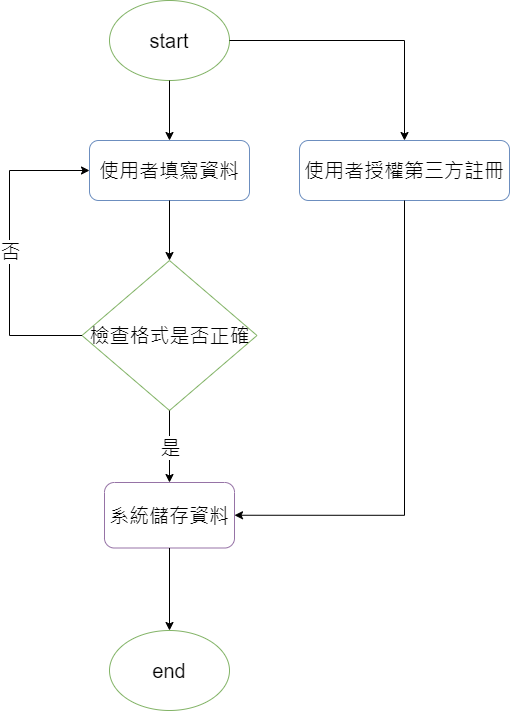
\includegraphics[width=0.5\textwidth]{assets/Process_Design/Register.png}
		\item 會員登入 \\
		      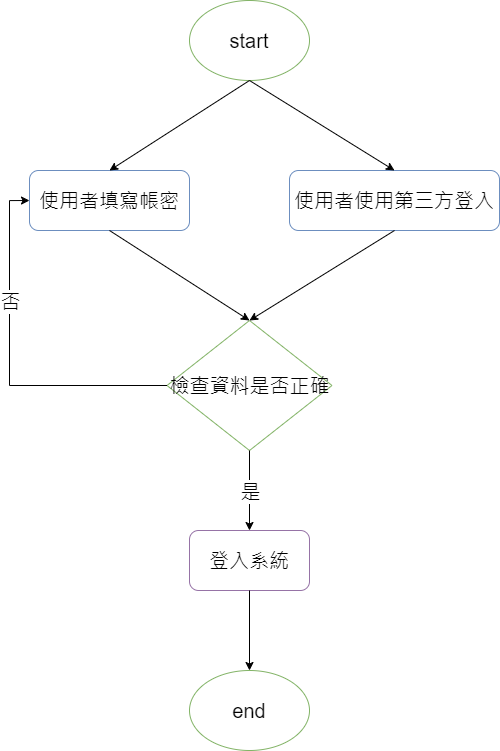
\includegraphics[width=0.5\textwidth]{assets/Process_Design/Login.png}
		\item 重設密碼 \\
		      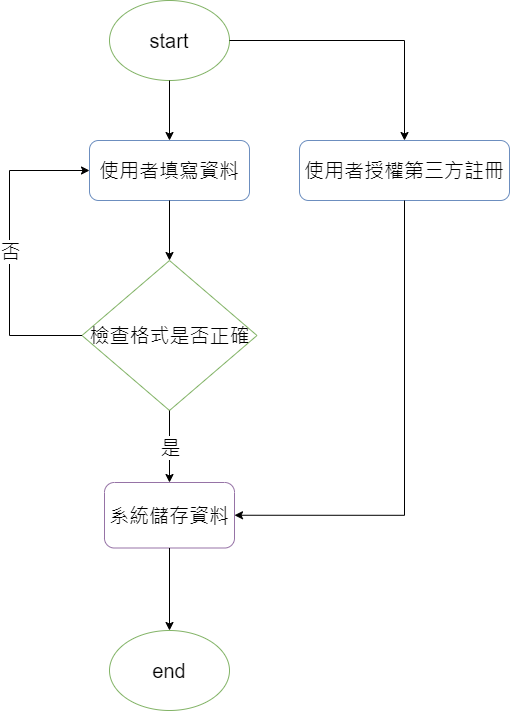
\includegraphics[width=0.5\textwidth]{assets/Process_Design/Register.png}
		\item 建立專案 \\
		      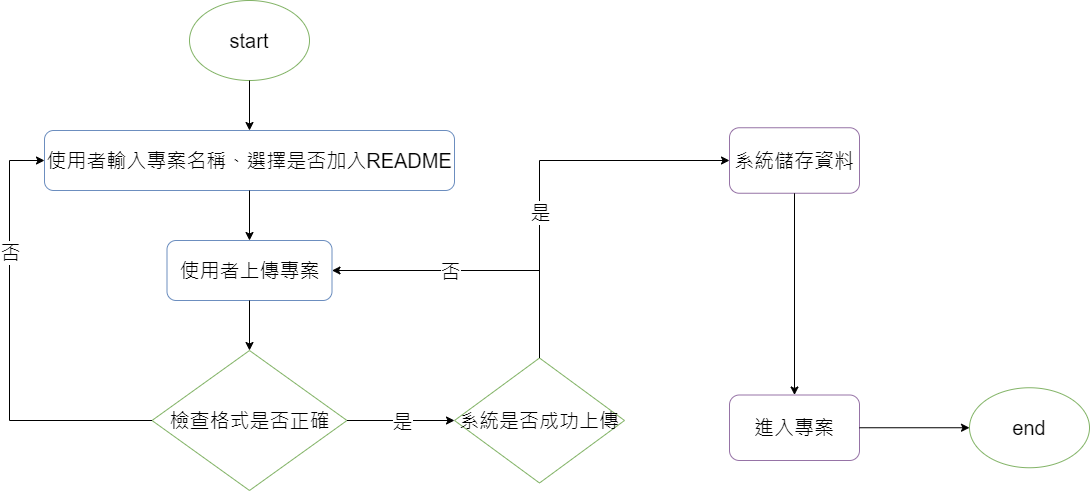
\includegraphics[width=0.8\textwidth]{assets/Process_Design/Create_Project.png}
		\item 編輯專案 \\
		      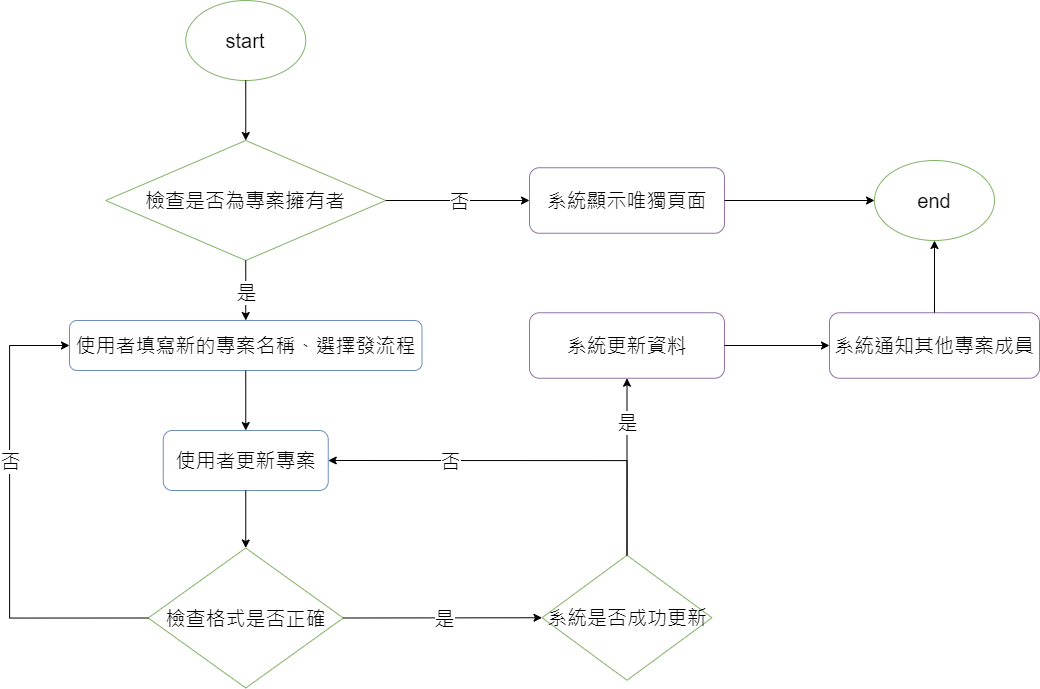
\includegraphics[width=0.8\textwidth]{assets/Process_Design/Edit_Project.png}
		\item 刪除專案 \\
		      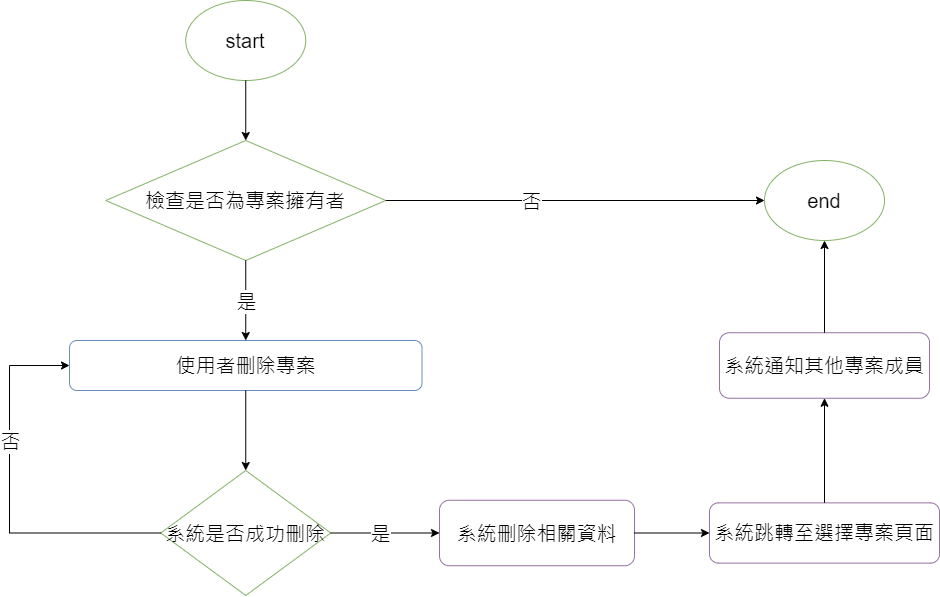
\includegraphics[width=0.8\textwidth]{assets/Process_Design/Delete_Project.png}
		\item 建立repository \\
		      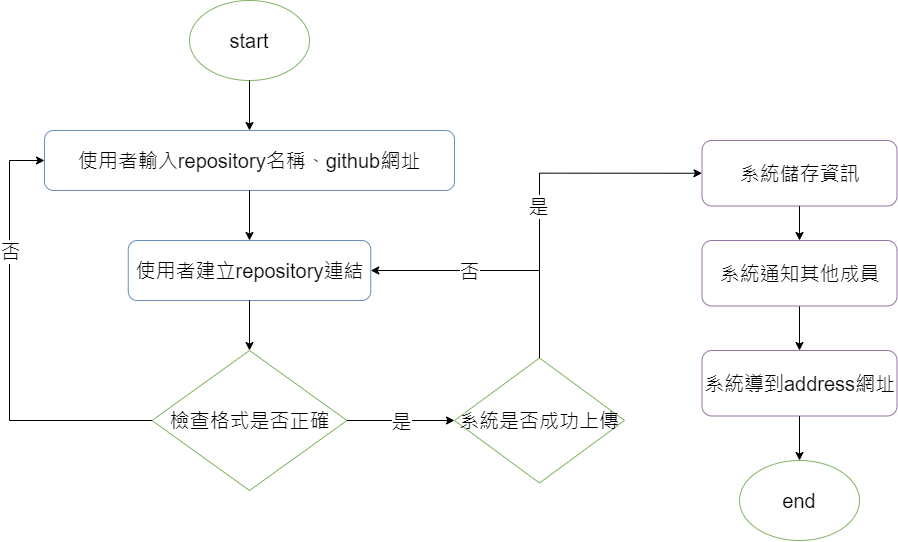
\includegraphics[width=0.8\textwidth]{assets/Process_Design/Create_repo.png}
		\item 刪除repository \\
		      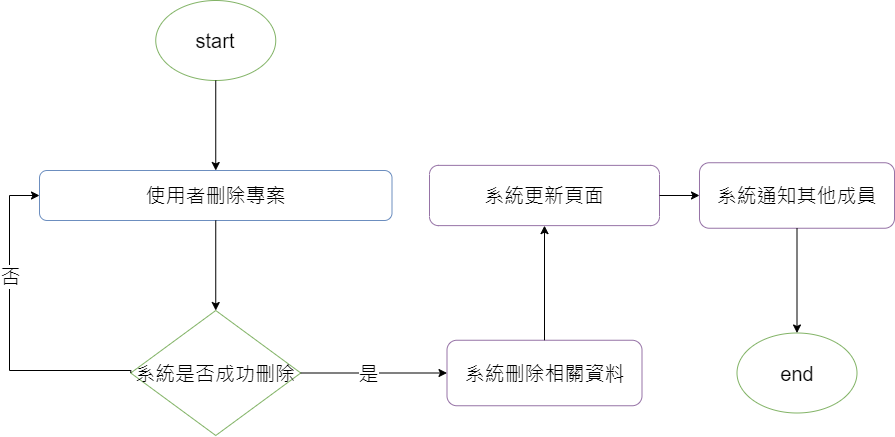
\includegraphics[width=0.8\textwidth]{assets/Process_Design/Delete_repo.png}
		\item 編輯文件 \\
		      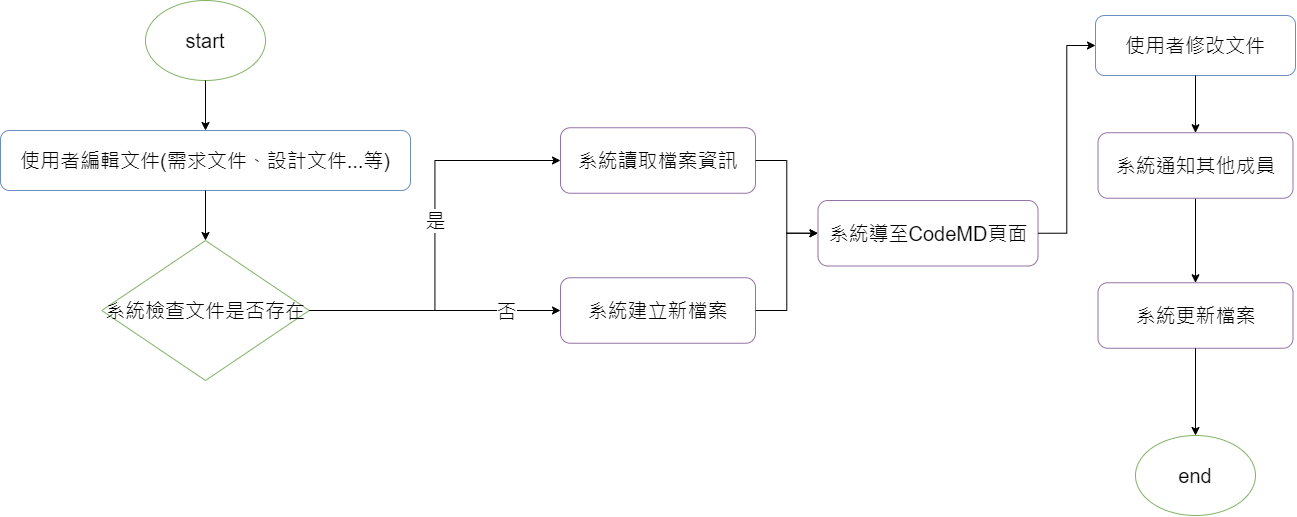
\includegraphics[width=0.8\textwidth]{assets/Process_Design/Edit_doc.png}
		\item 預覽文件 \\
		      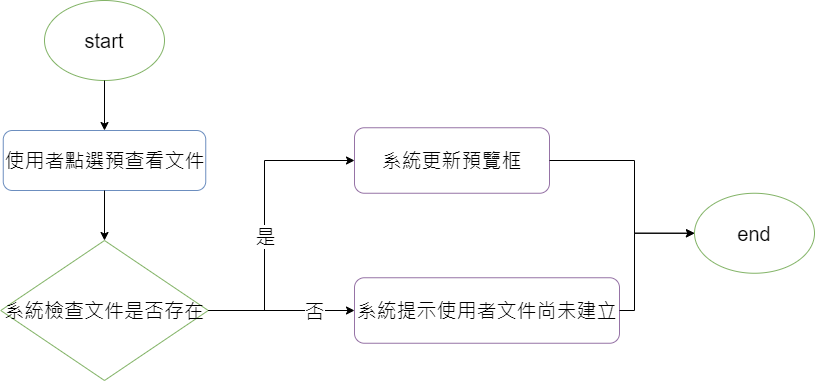
\includegraphics[width=0.8\textwidth]{assets/Process_Design/Preview_doc.png}
		\item 看板新增任務 \\
		      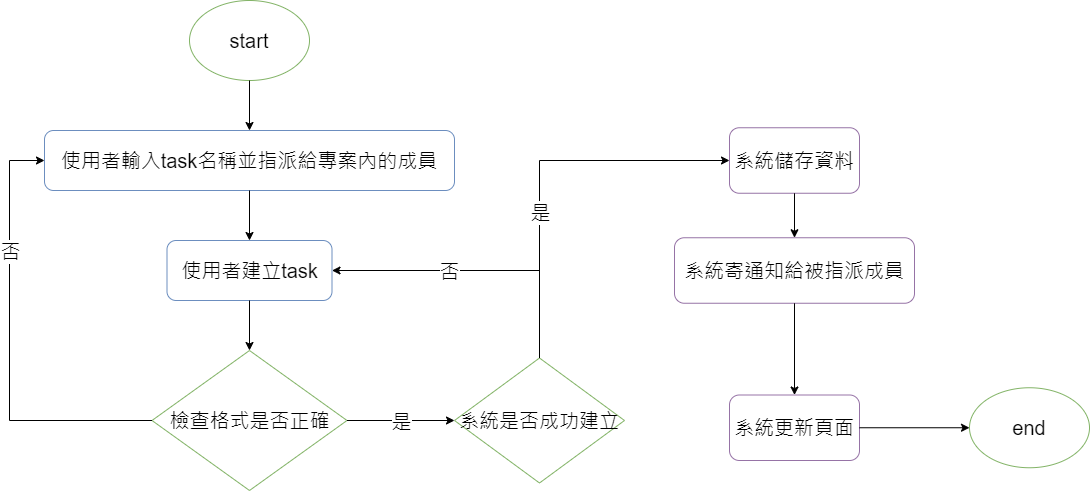
\includegraphics[width=0.8\textwidth]{assets/Process_Design/Create_task.png}
		\item 看板編輯任務 \\
		      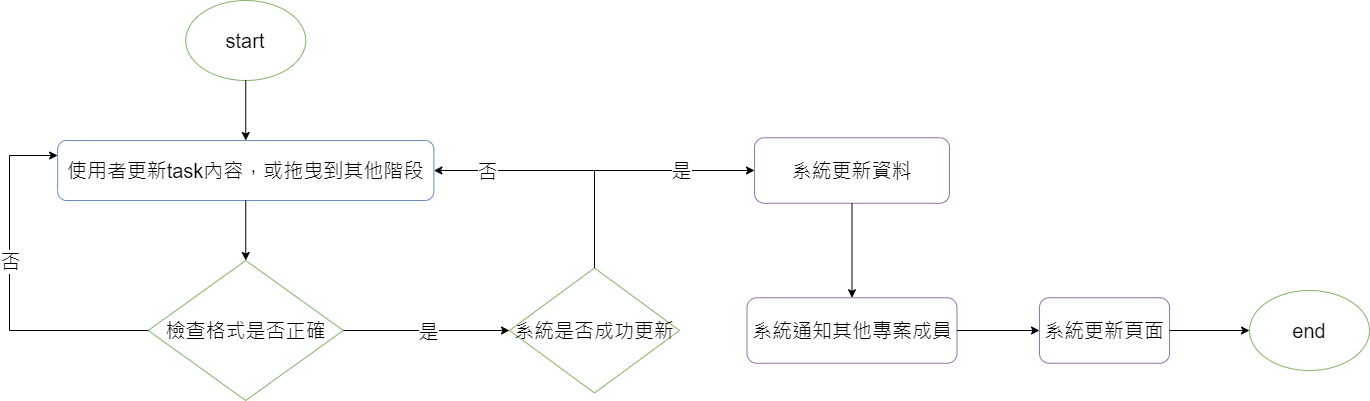
\includegraphics[width=0.8\textwidth]{assets/Process_Design/Edit_task.png}
		\item 看板刪除任務 \\
		      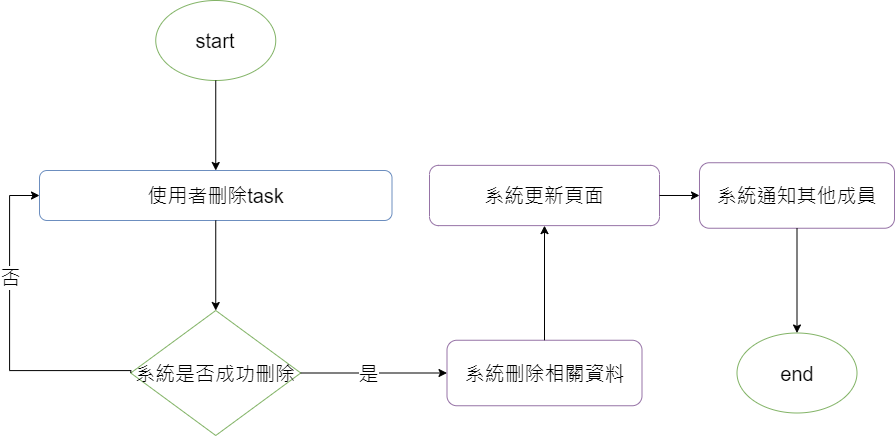
\includegraphics[width=0.5\textwidth]{assets/Process_Design/Delete_task.png}
		\item Q\&A文件\\
		      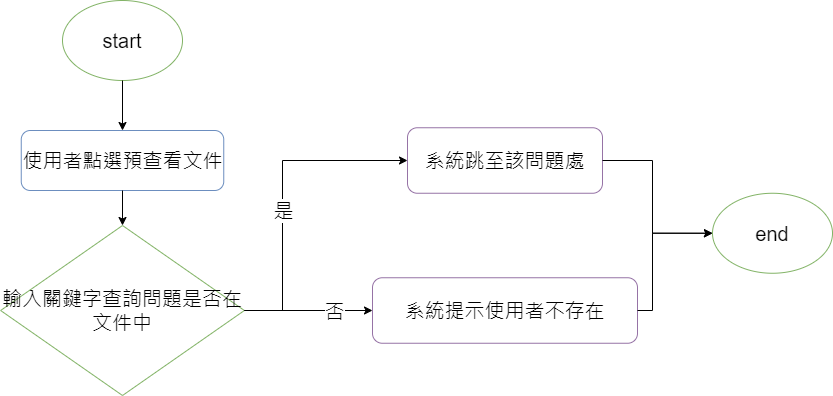
\includegraphics[width=0.8\textwidth]{assets/Process_Design/QA_doc.png}
		\item 變更成員 \\
		      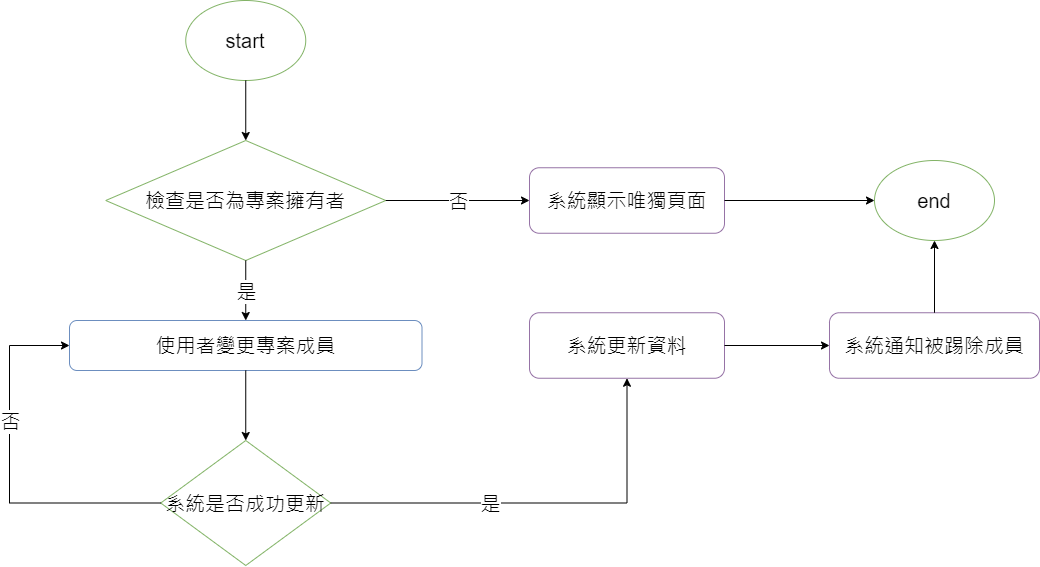
\includegraphics[width=0.8\textwidth]{assets/Process_Design/Change_Members.png}
		\item 邀請其他人 \\
		      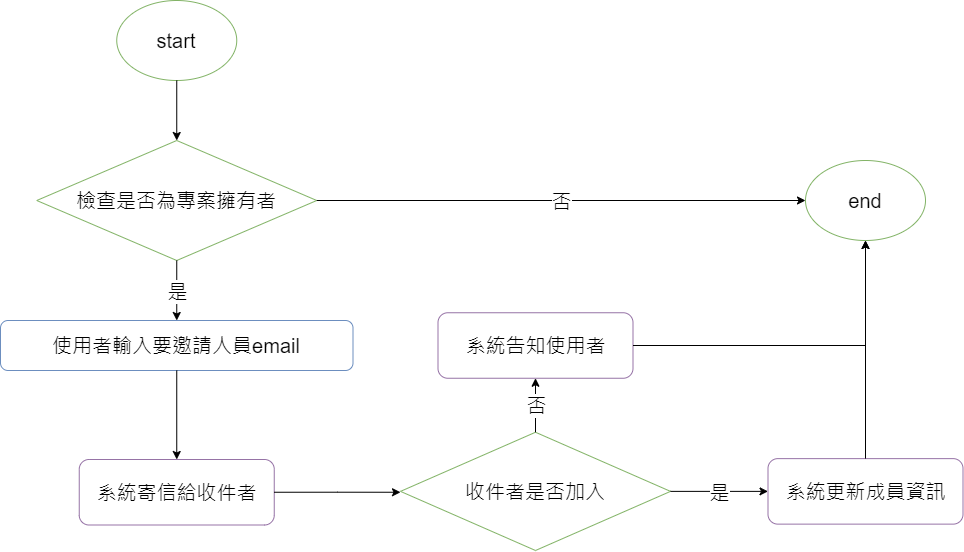
\includegraphics[width=0.8\textwidth]{assets/Process_Design/Join_Project.png}
		\item 邀請其他人 \\
		      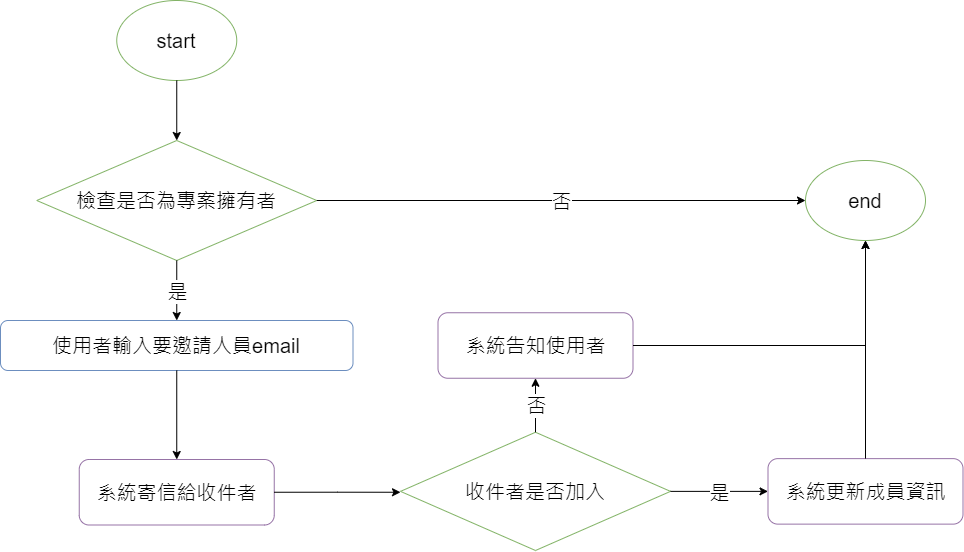
\includegraphics[width=0.8\textwidth]{assets/Process_Design/Join_Project.png}
		\item 設定個人資料 \\
		      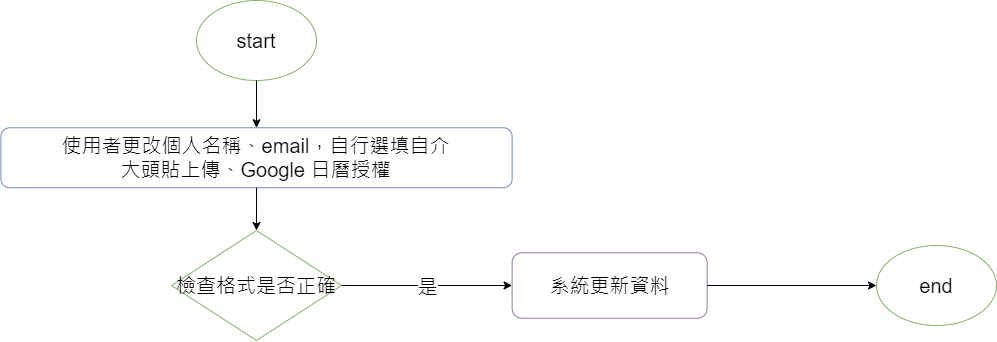
\includegraphics[width=0.8\textwidth]{assets/Process_Design/Set_Profile.png}
	\end{enumerate}
\end{obeylines}

\section*{4. 使用者畫面設計(User Interface Design)}

% \begin{obeylines}
% 	\parindent=0pt
% 	可用各種畫面設計方式,如發展網頁prototype、繪製PowerPoint投影片等,去設計你的主要系統畫面。此部份應是SRS中使用者介面分析的進階設計版本。
% 	線框圖? 包含所有UI設計 版型顏色等等
% 	CLI工具UI設計
% 	何
% \end{obeylines}

\begin{enumerate}
	\item User 登入 \\ 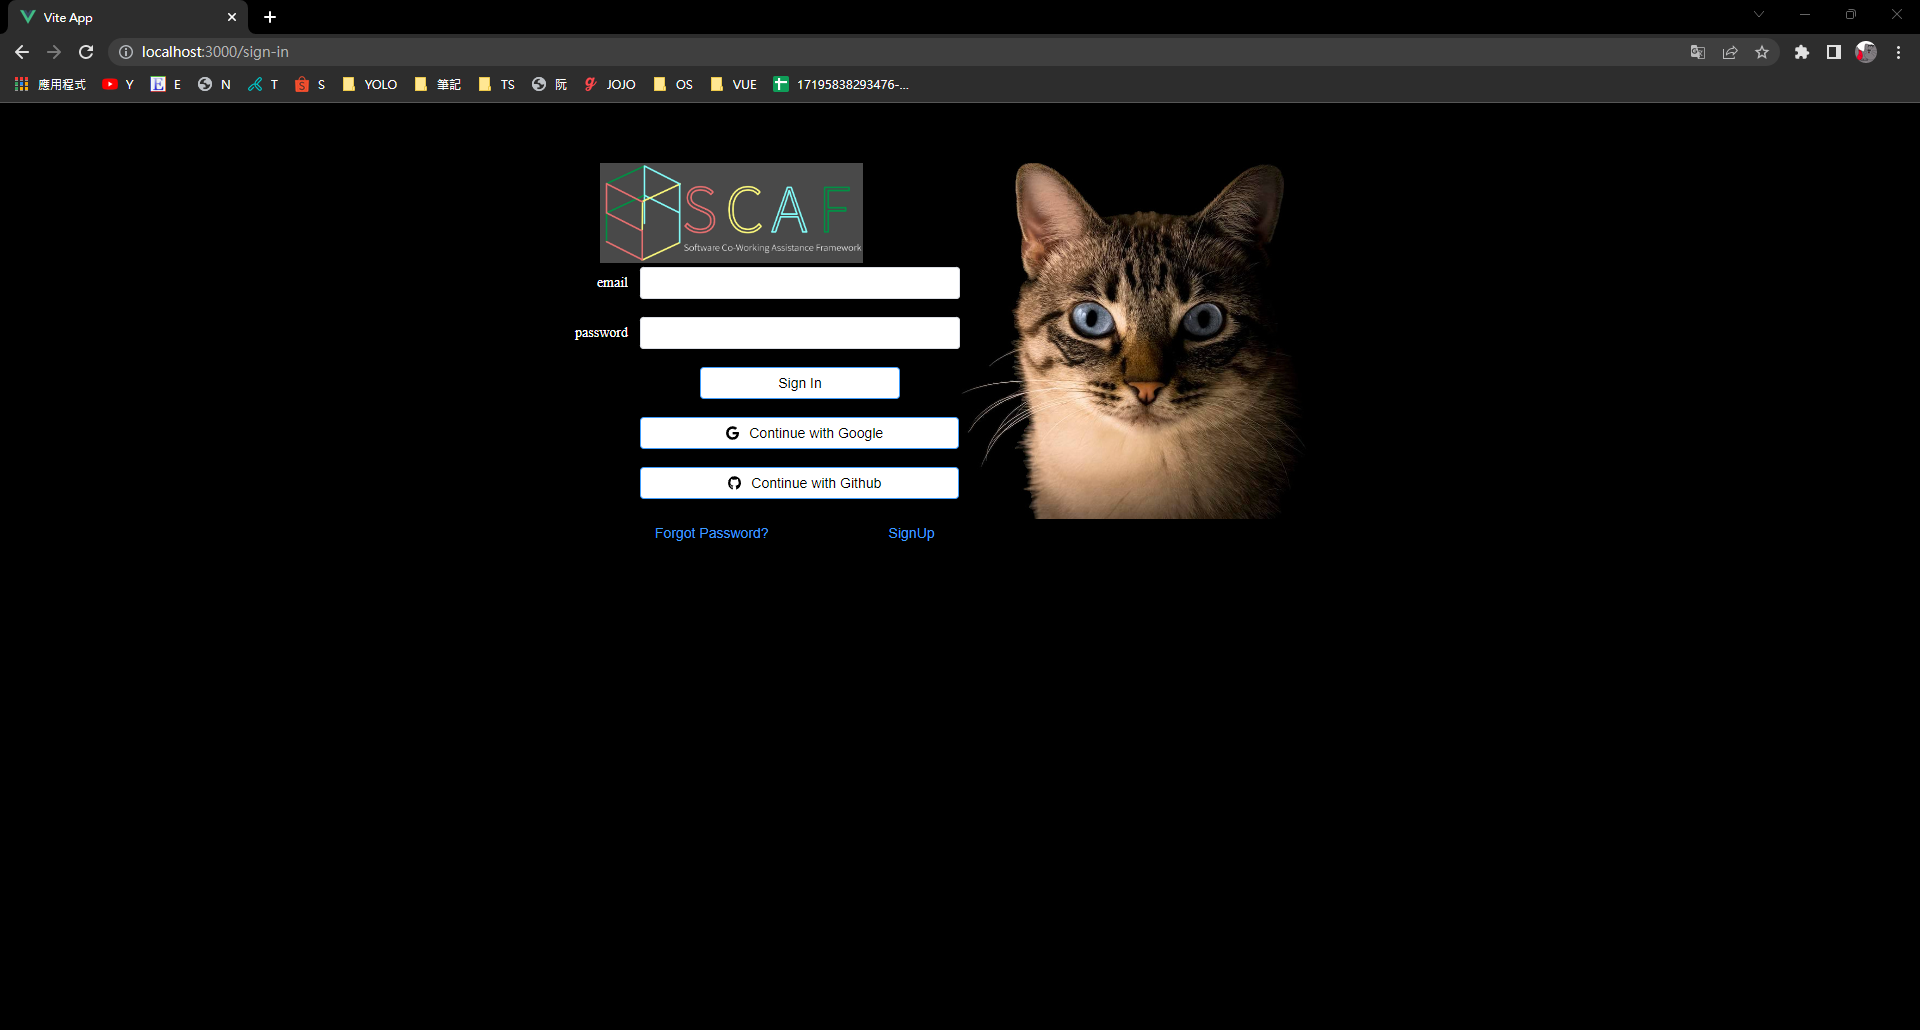
\includegraphics[width=0.9\textwidth]{assets/UI/signin.png}
	\item User 註冊 \\ 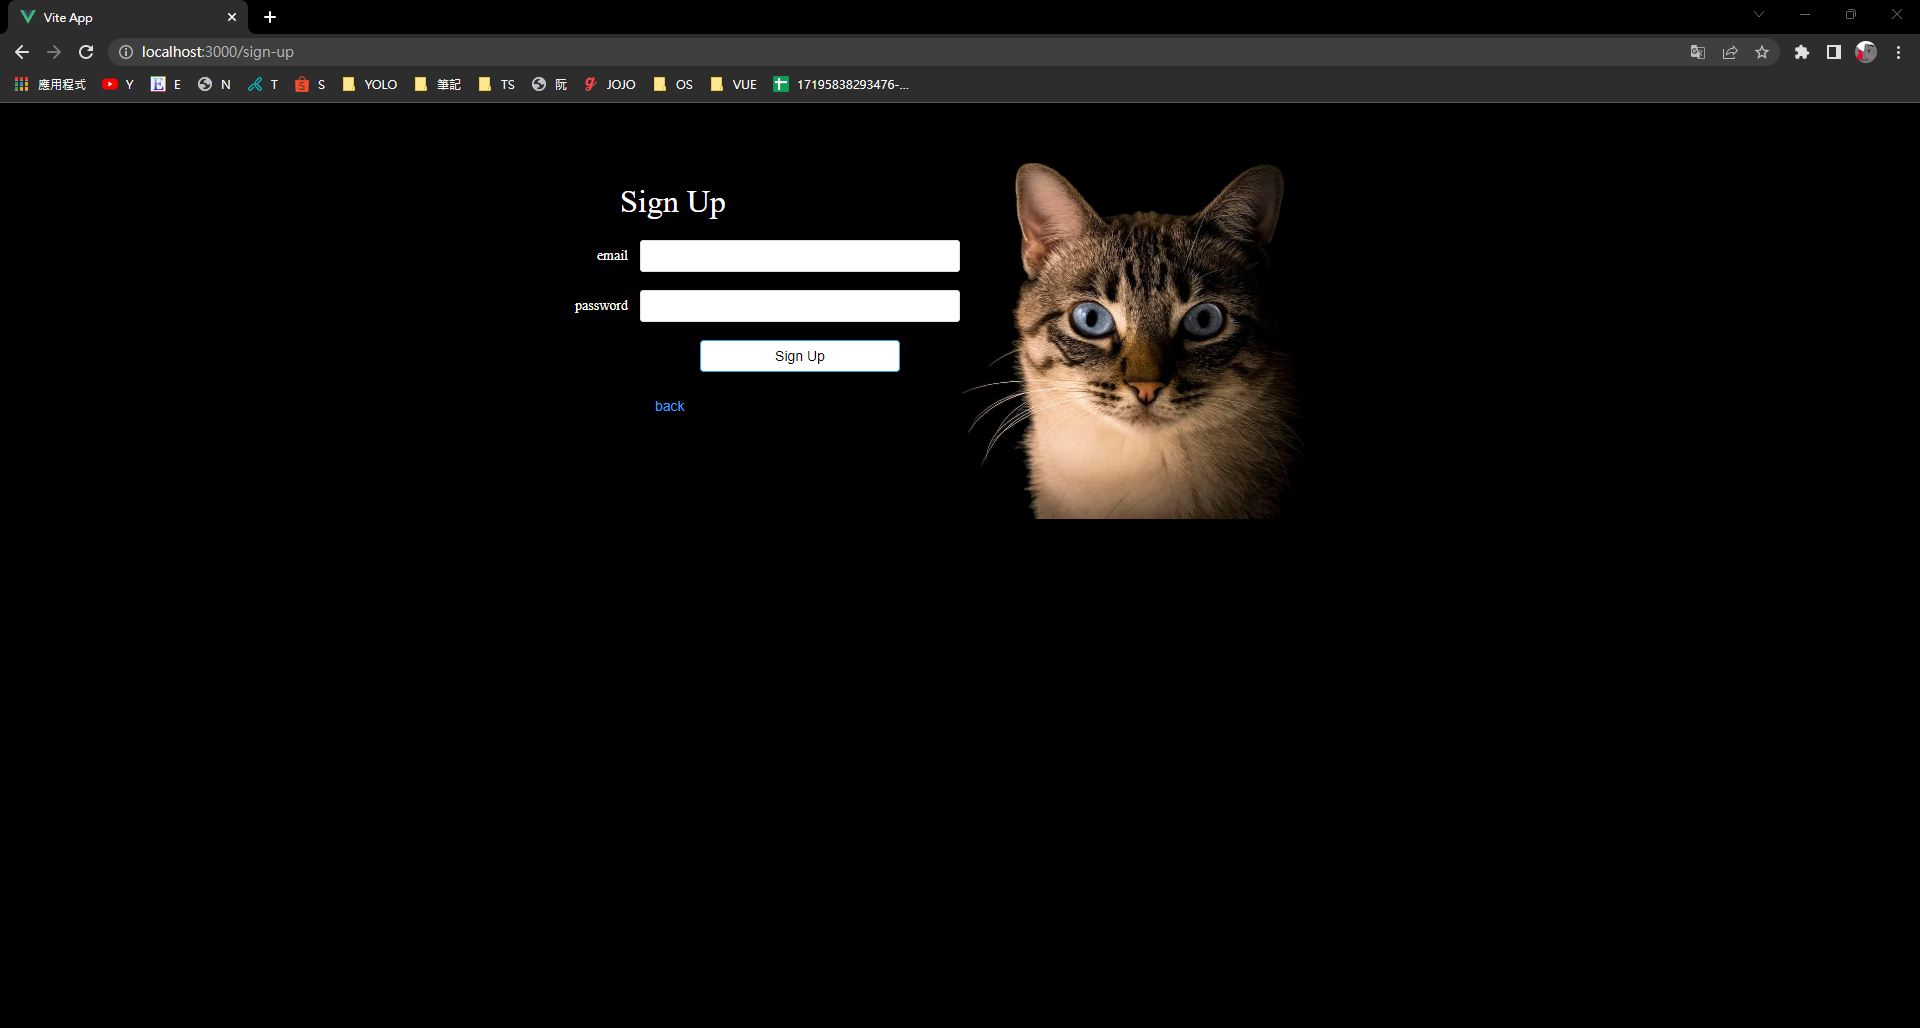
\includegraphics[width=0.9\textwidth]{assets/UI/signup.png}
	\item 個人設定 \\ 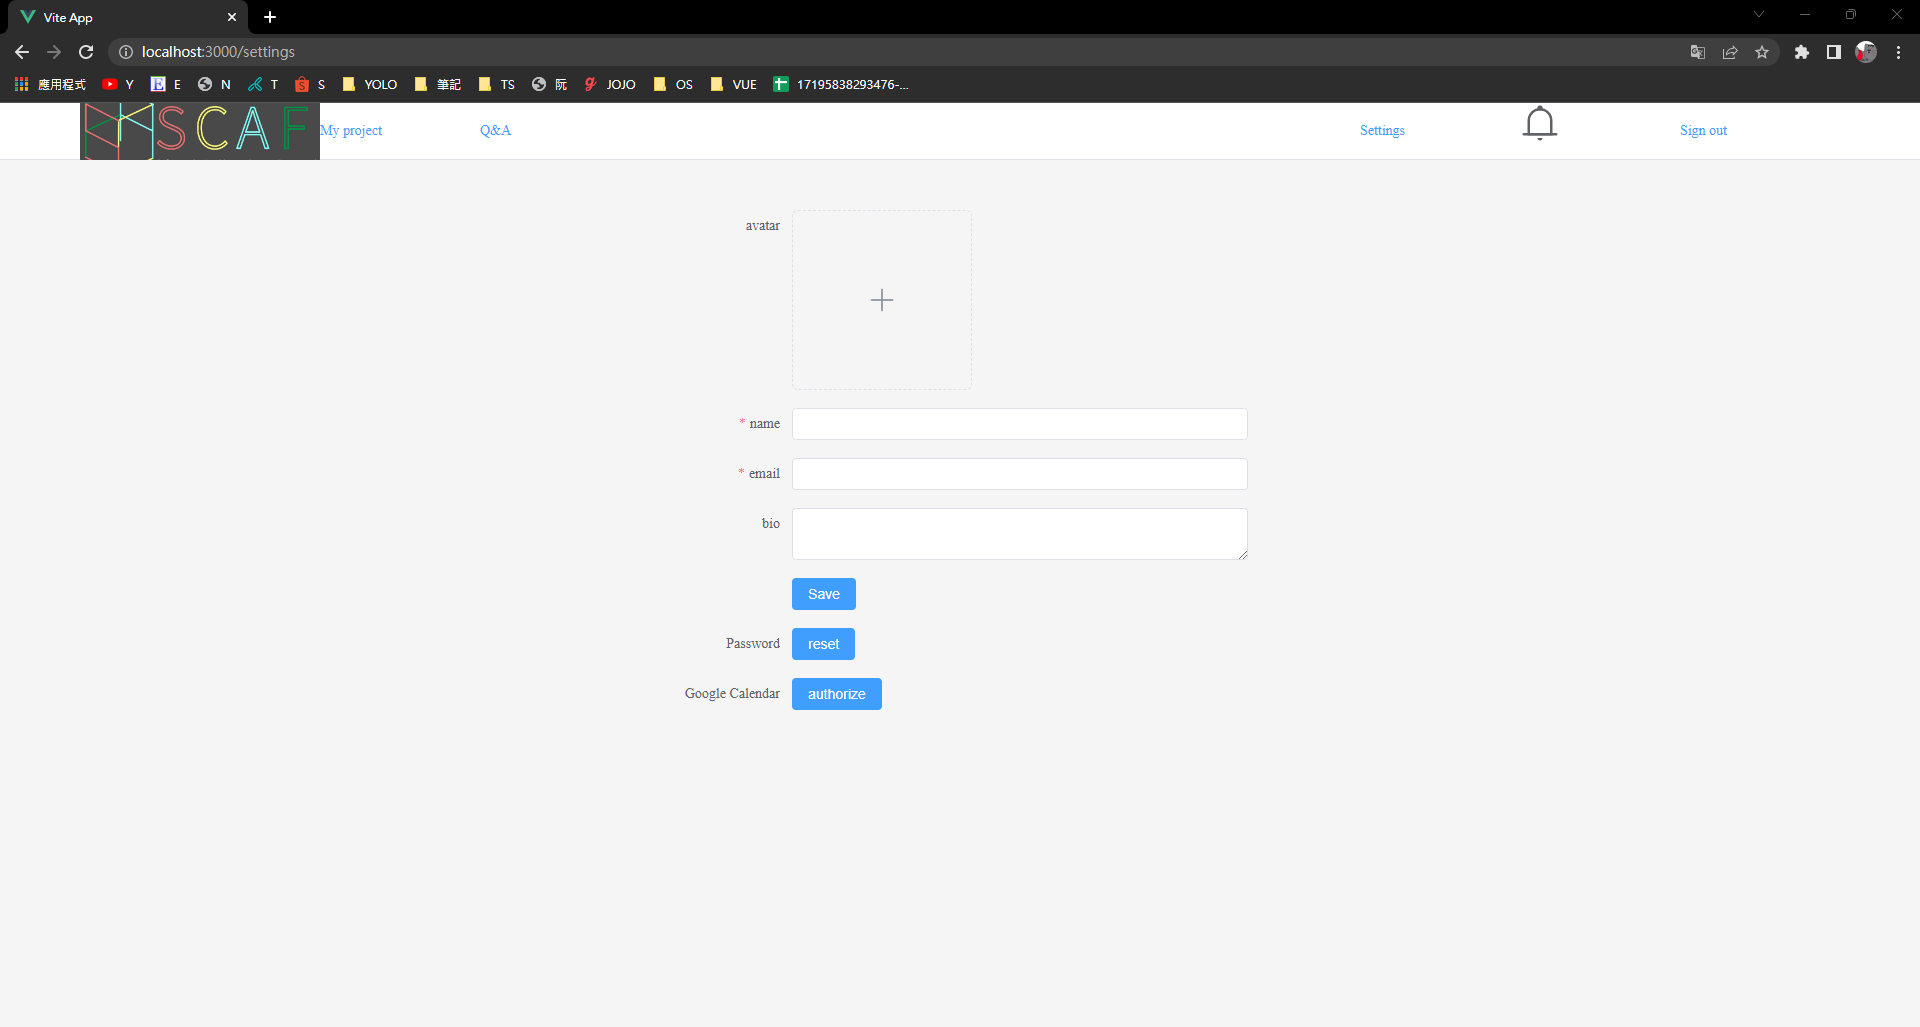
\includegraphics[width=0.9\textwidth]{assets/UI/settings.png}
	\item 忘記密碼 \\ 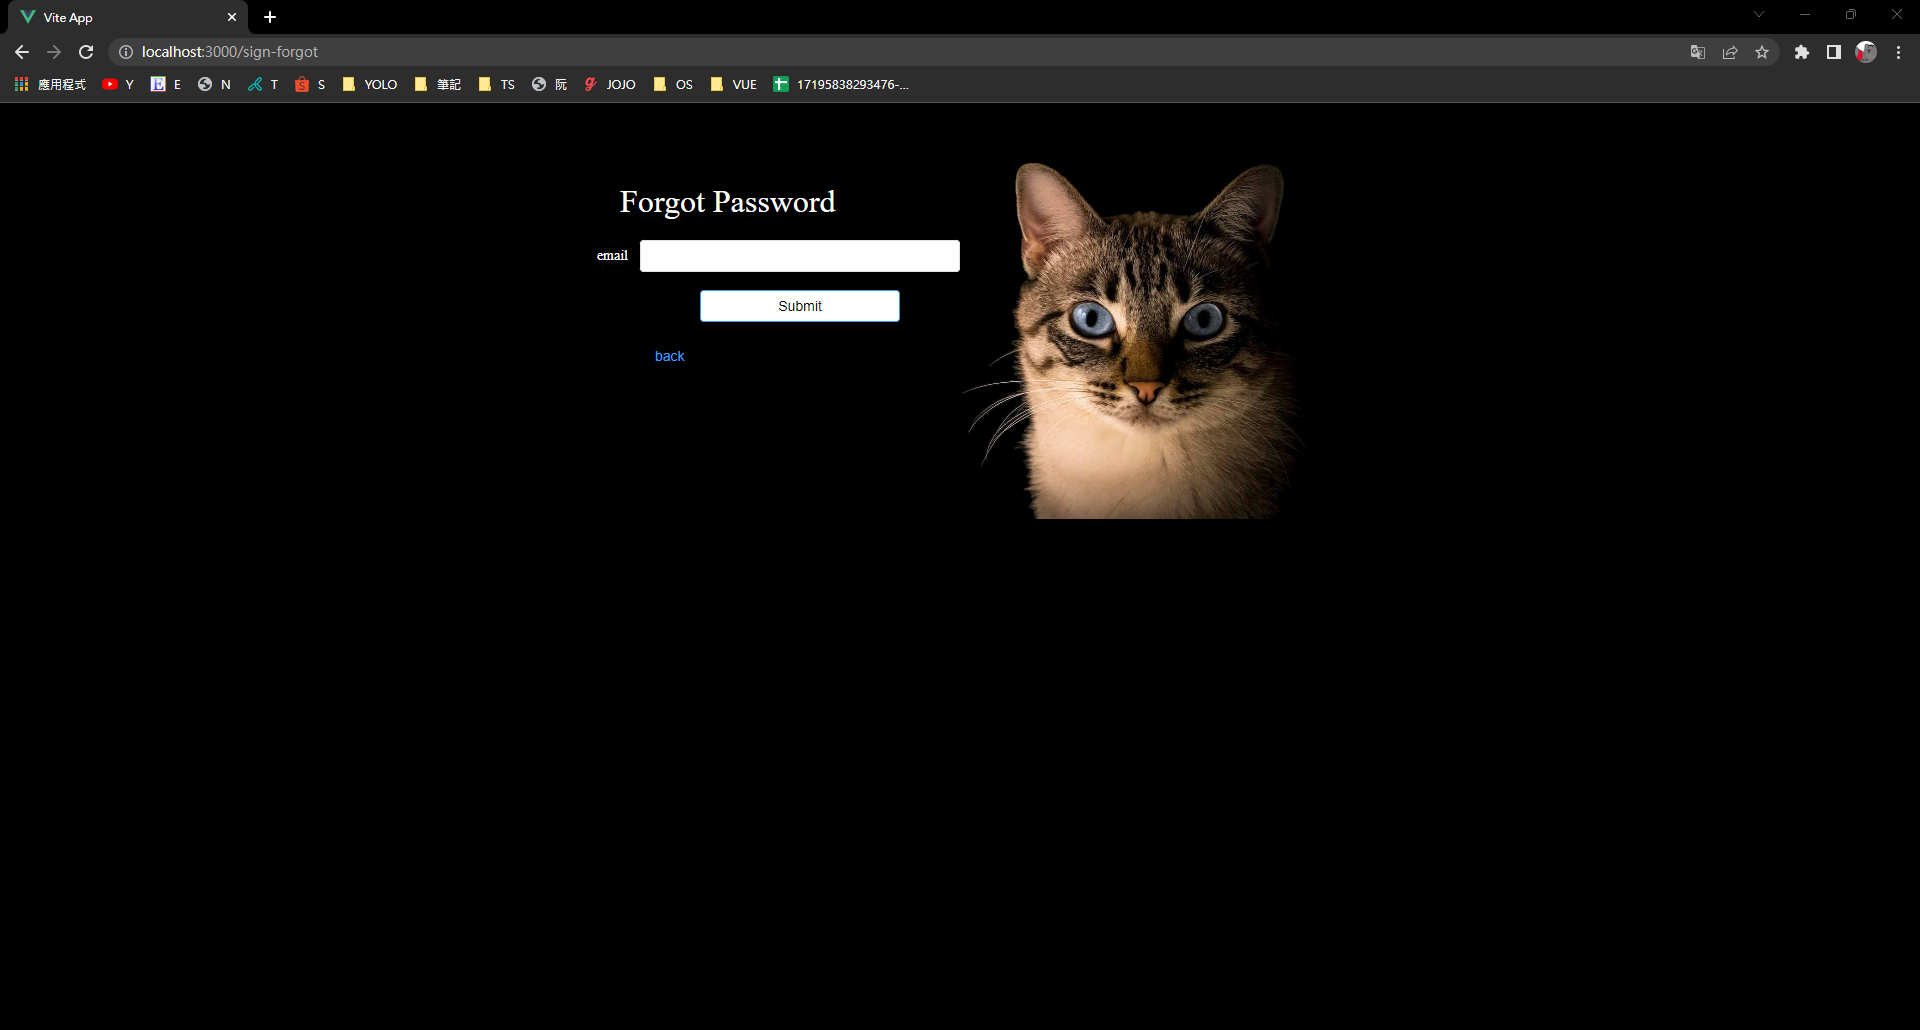
\includegraphics[width=0.9\textwidth]{assets/UI/forgot.png}
	\item 通知 \\ 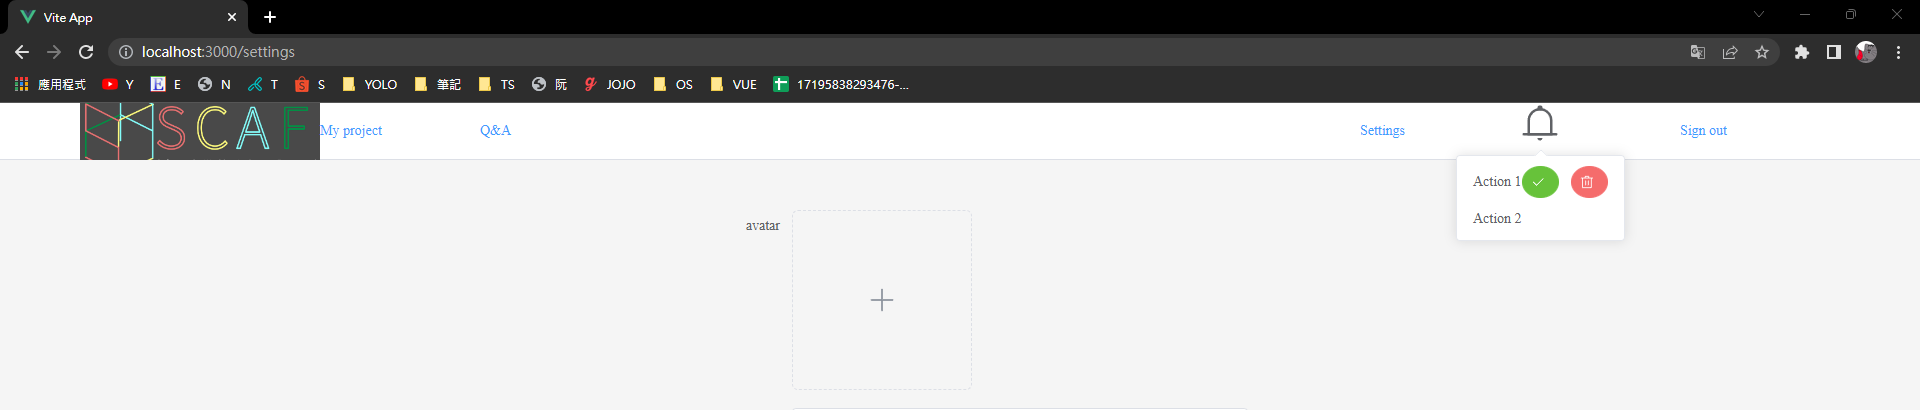
\includegraphics[width=0.9\textwidth]{assets/UI/notify.png}
	\item Projects 頁面 \\ 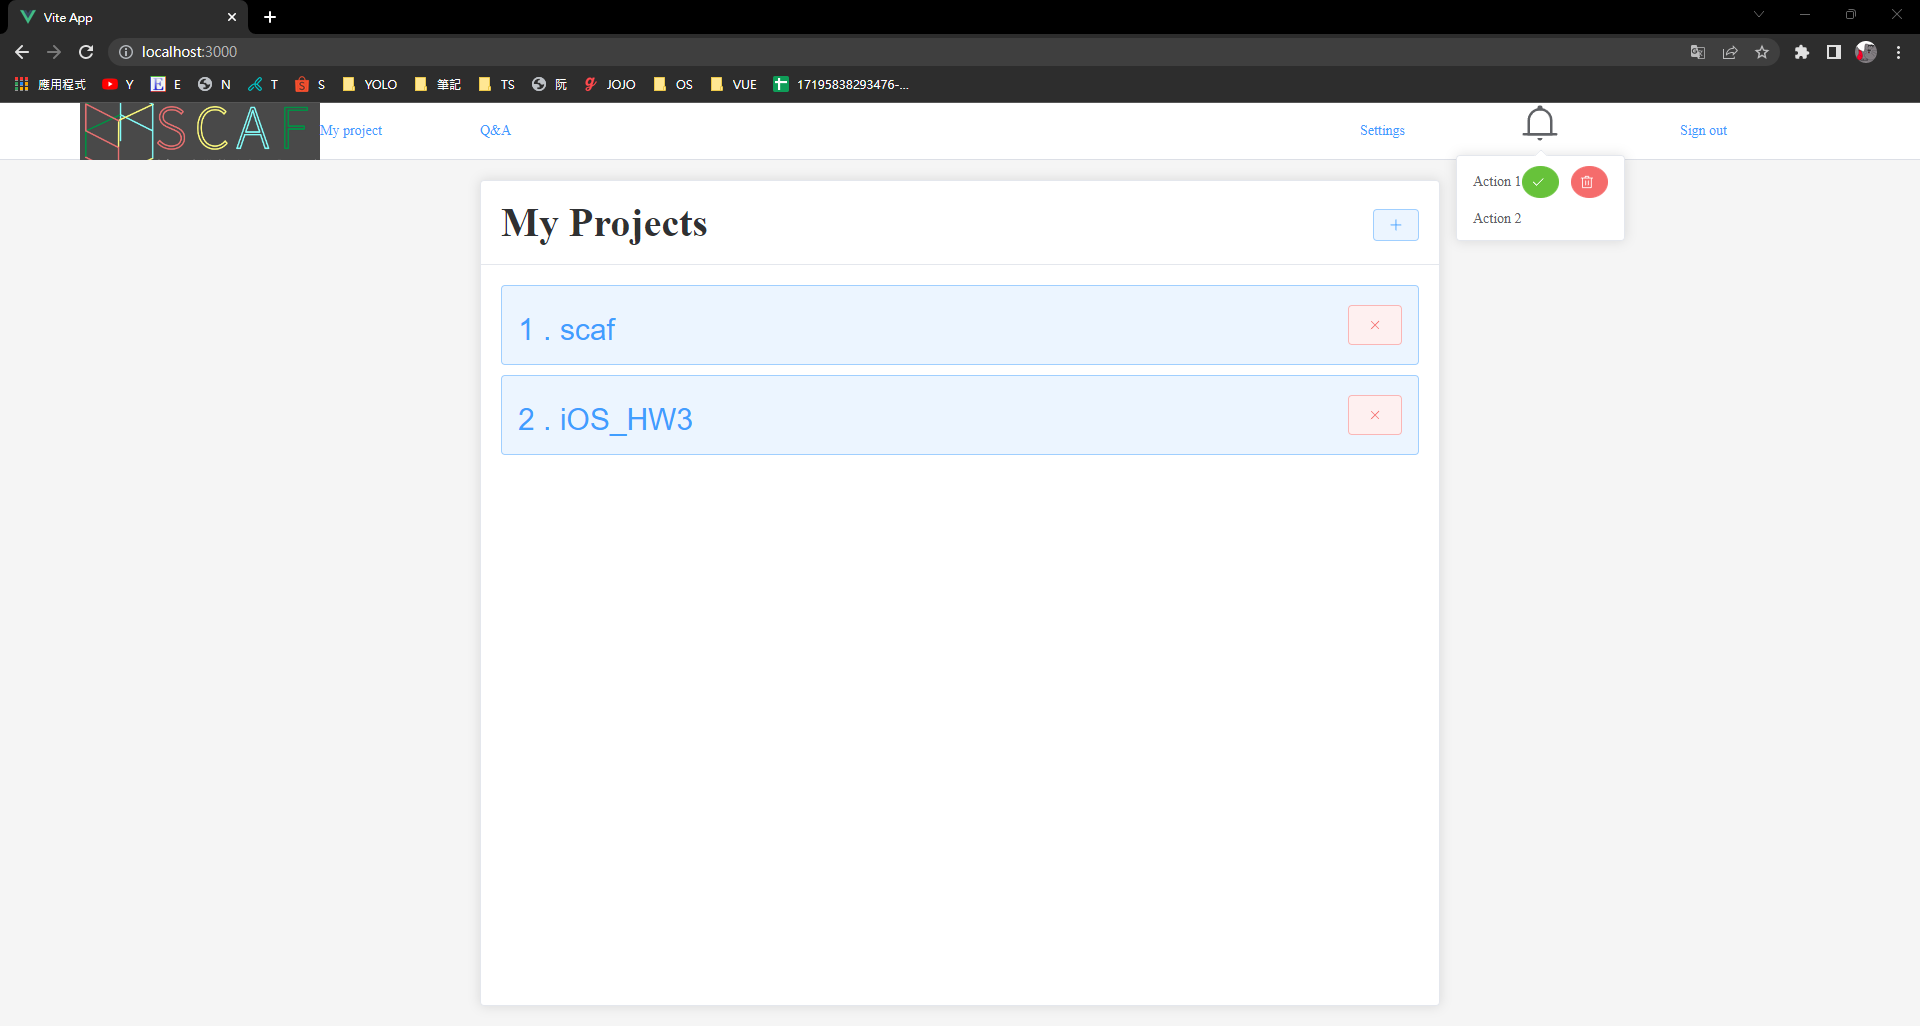
\includegraphics[width=0.9\textwidth]{assets/UI/projects.png}
	\item 專案設定 \\ 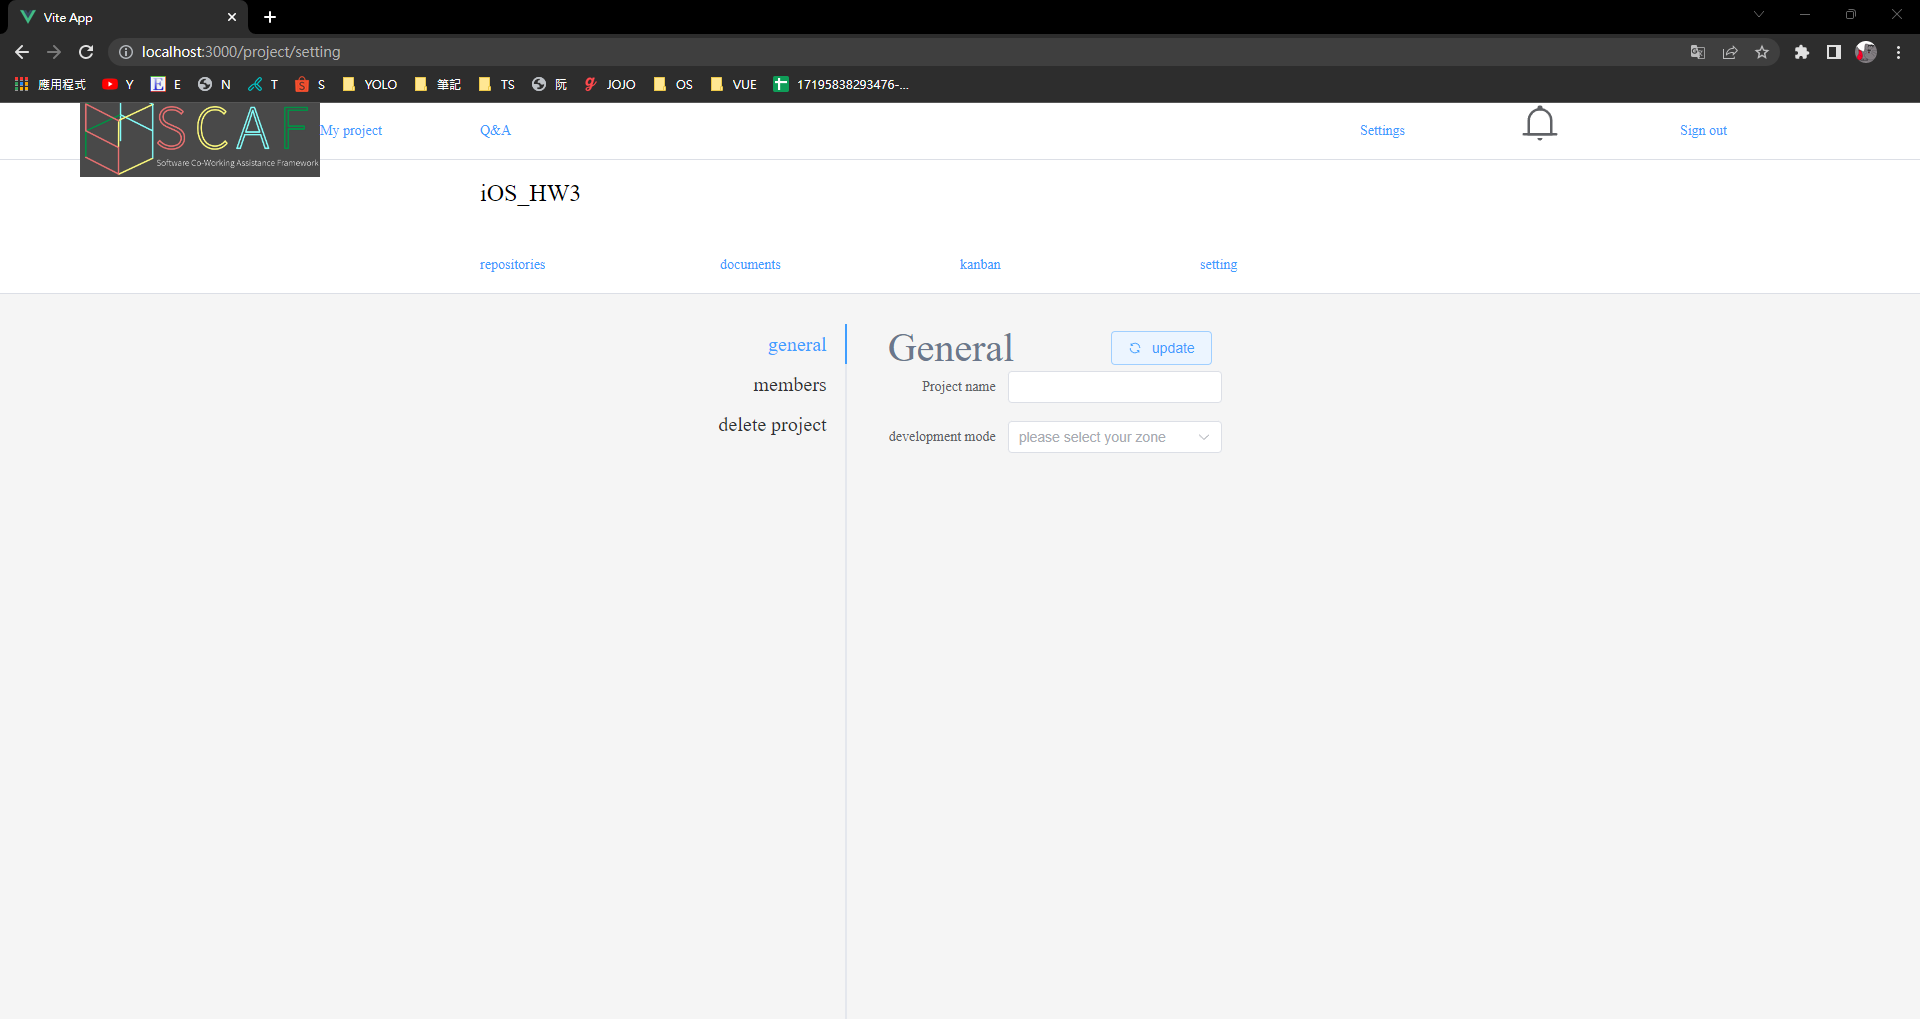
\includegraphics[width=0.9\textwidth]{assets/UI/project_setting.png}
	\item 專案 Repo \\ 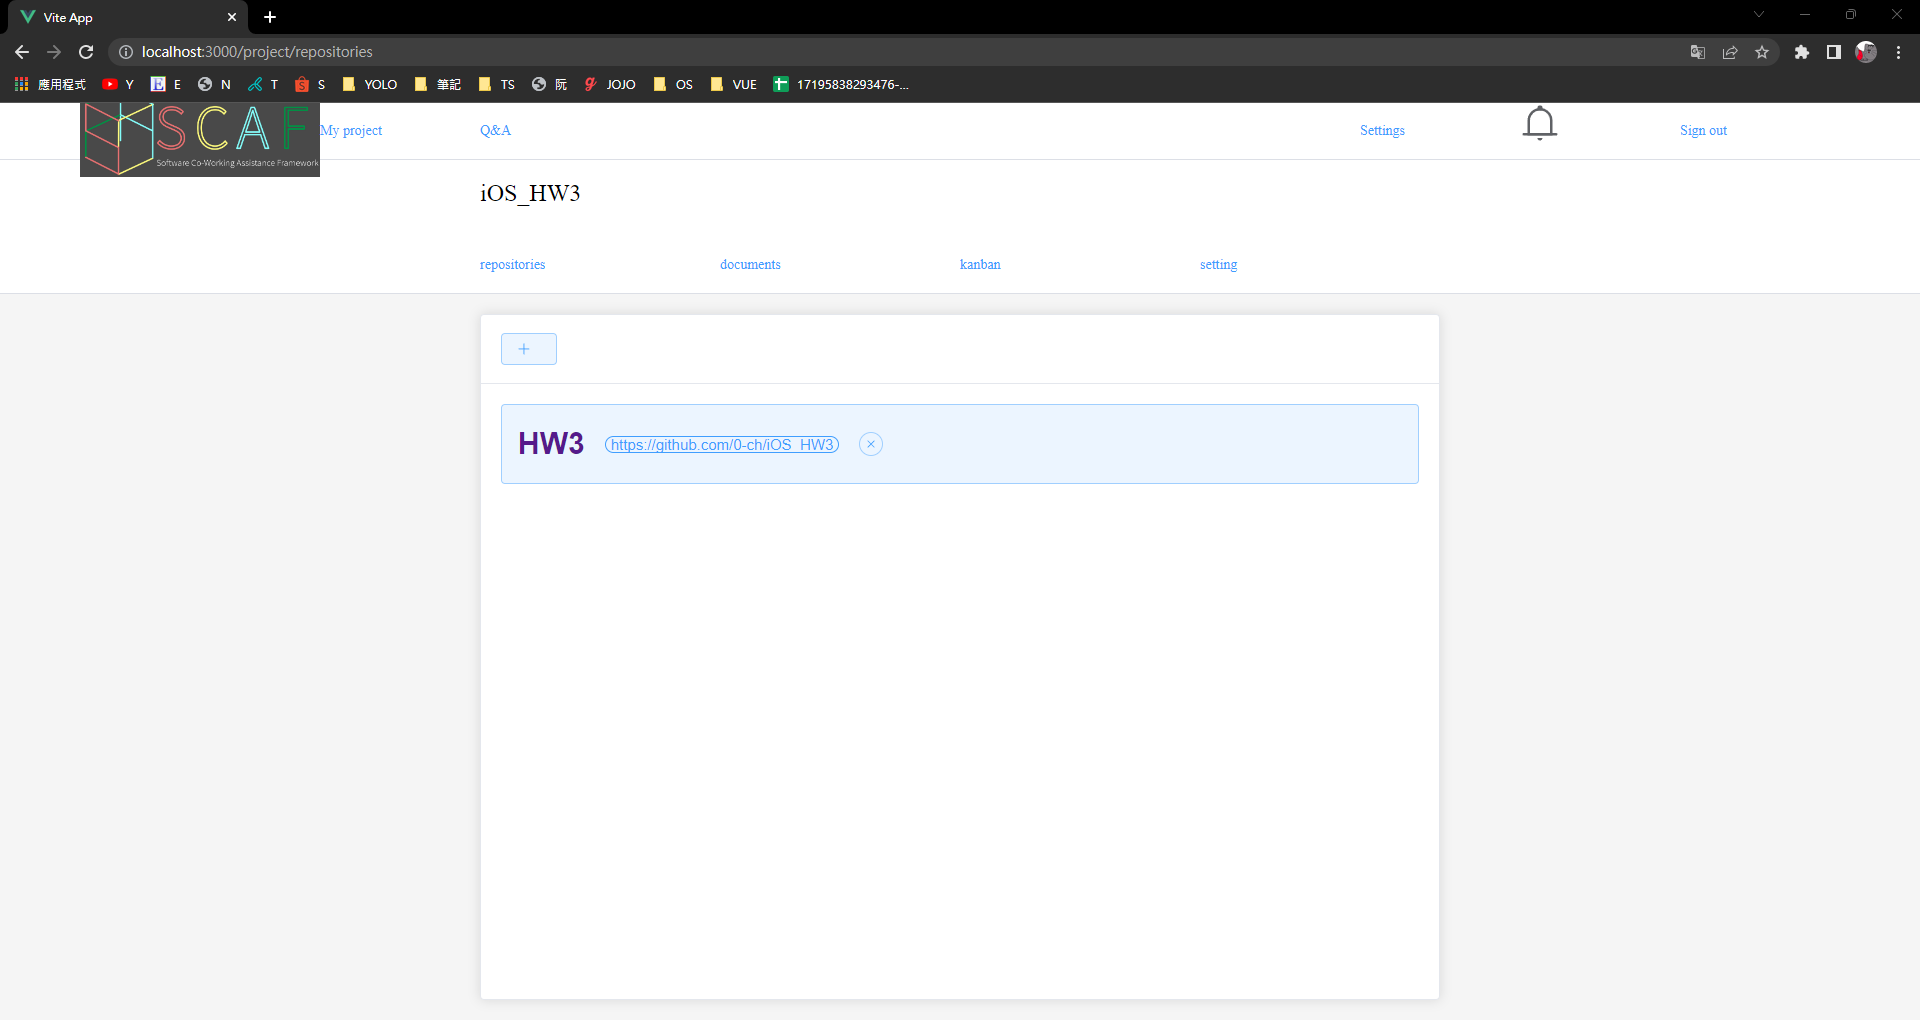
\includegraphics[width=0.9\textwidth]{assets/UI/repo.png}
	\item 新增 Repo \\ 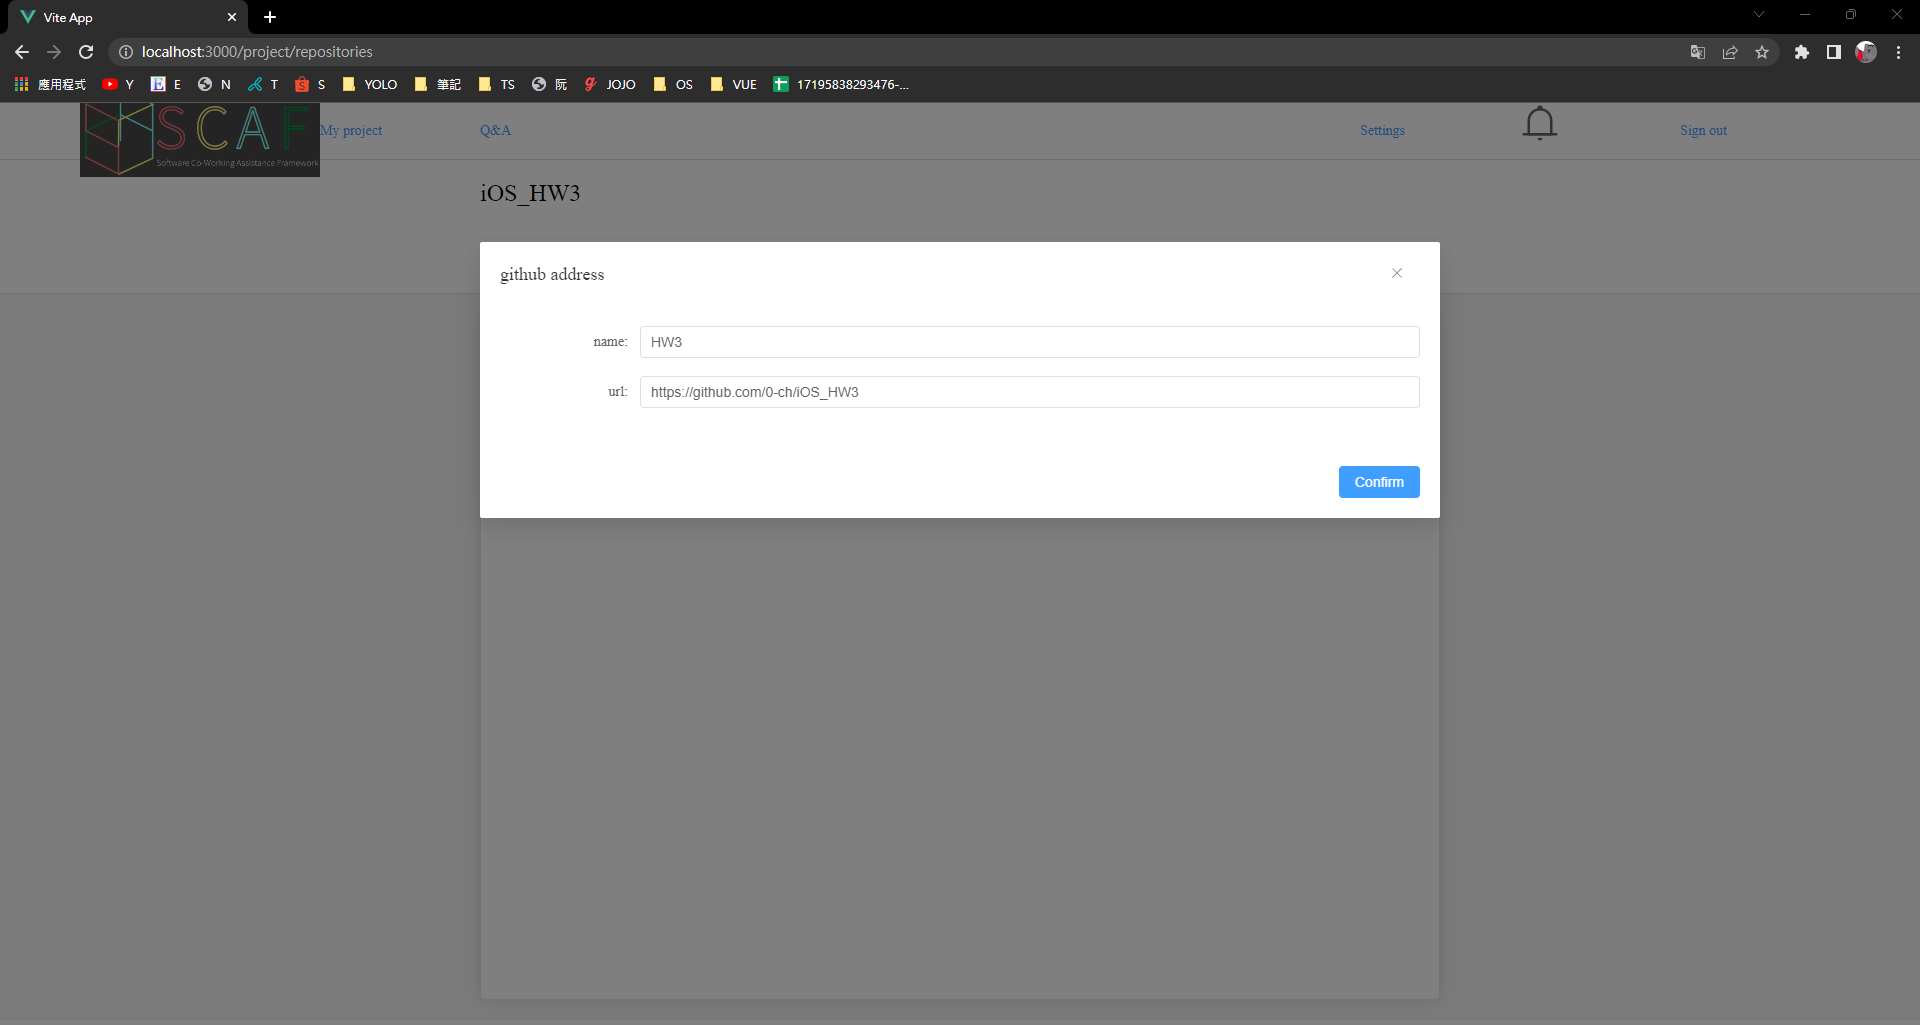
\includegraphics[width=0.9\textwidth]{assets/UI/add_repo.png}
	\item 專案成員 \\ 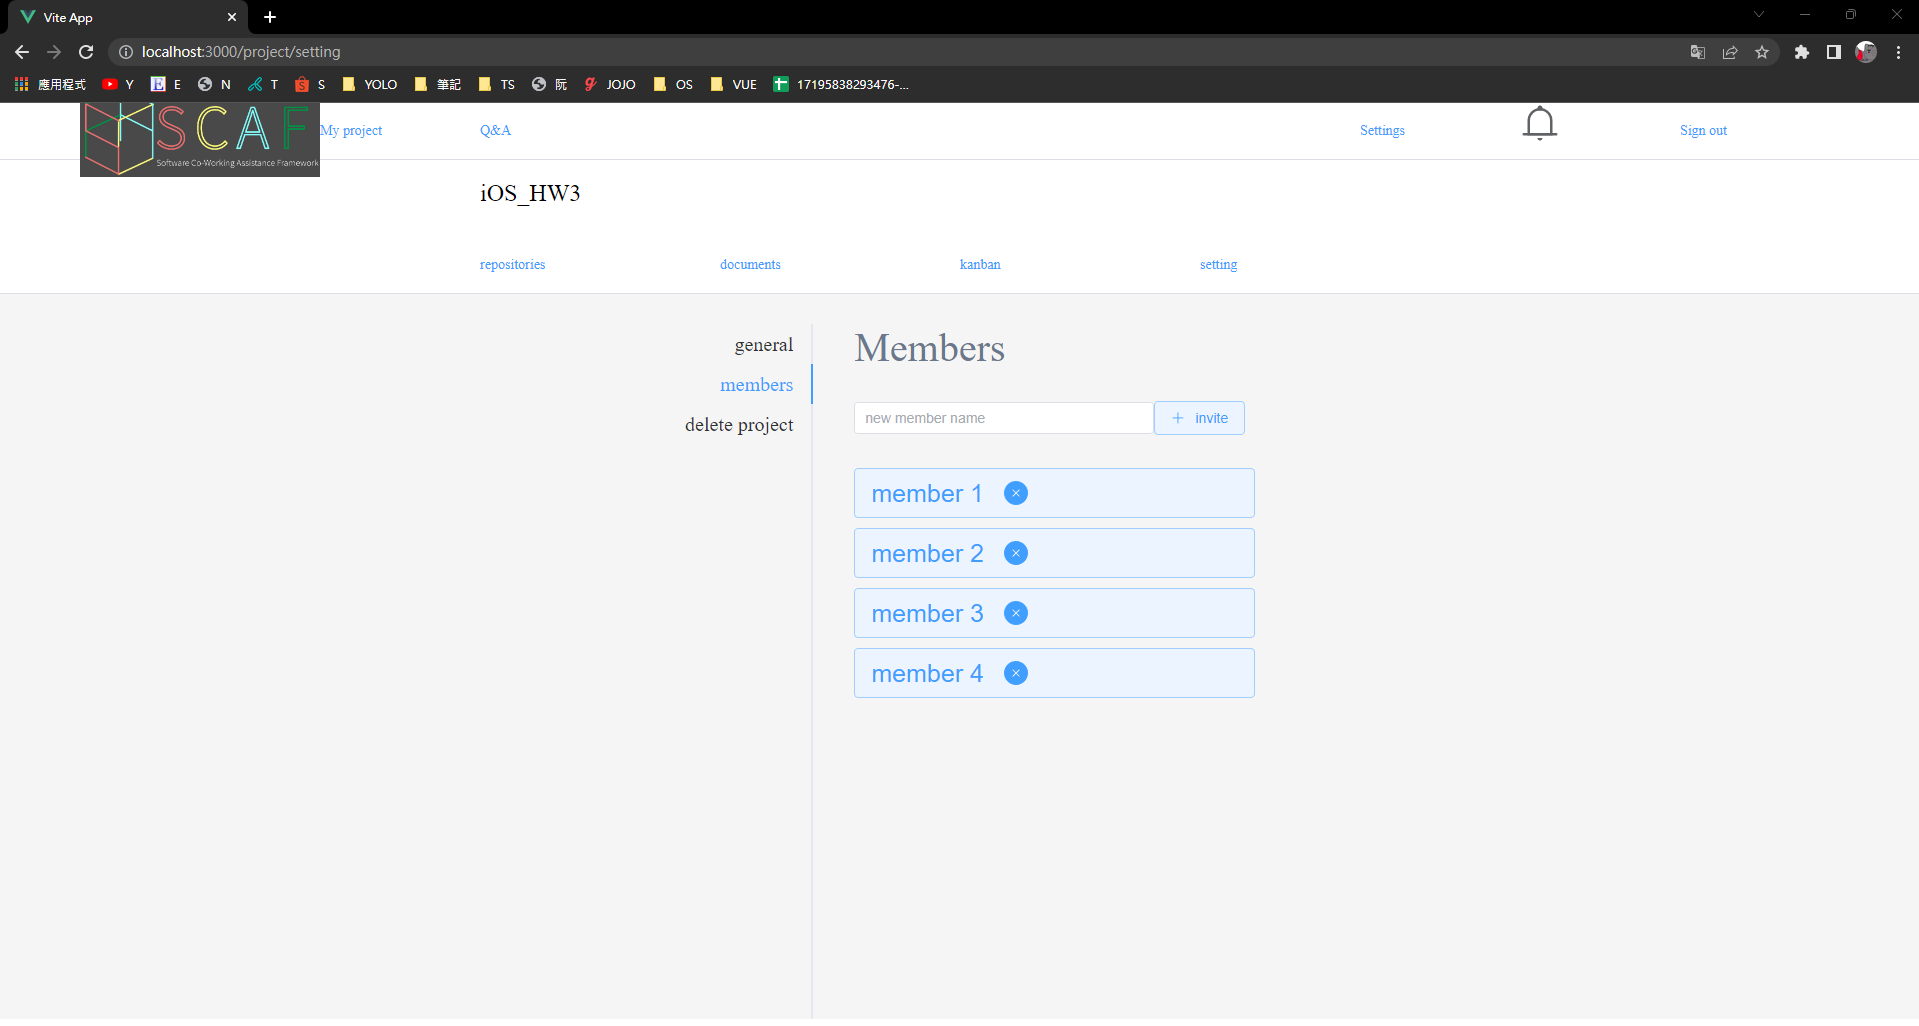
\includegraphics[width=0.9\textwidth]{assets/UI/member.png}
	\item 專案看板 \\ 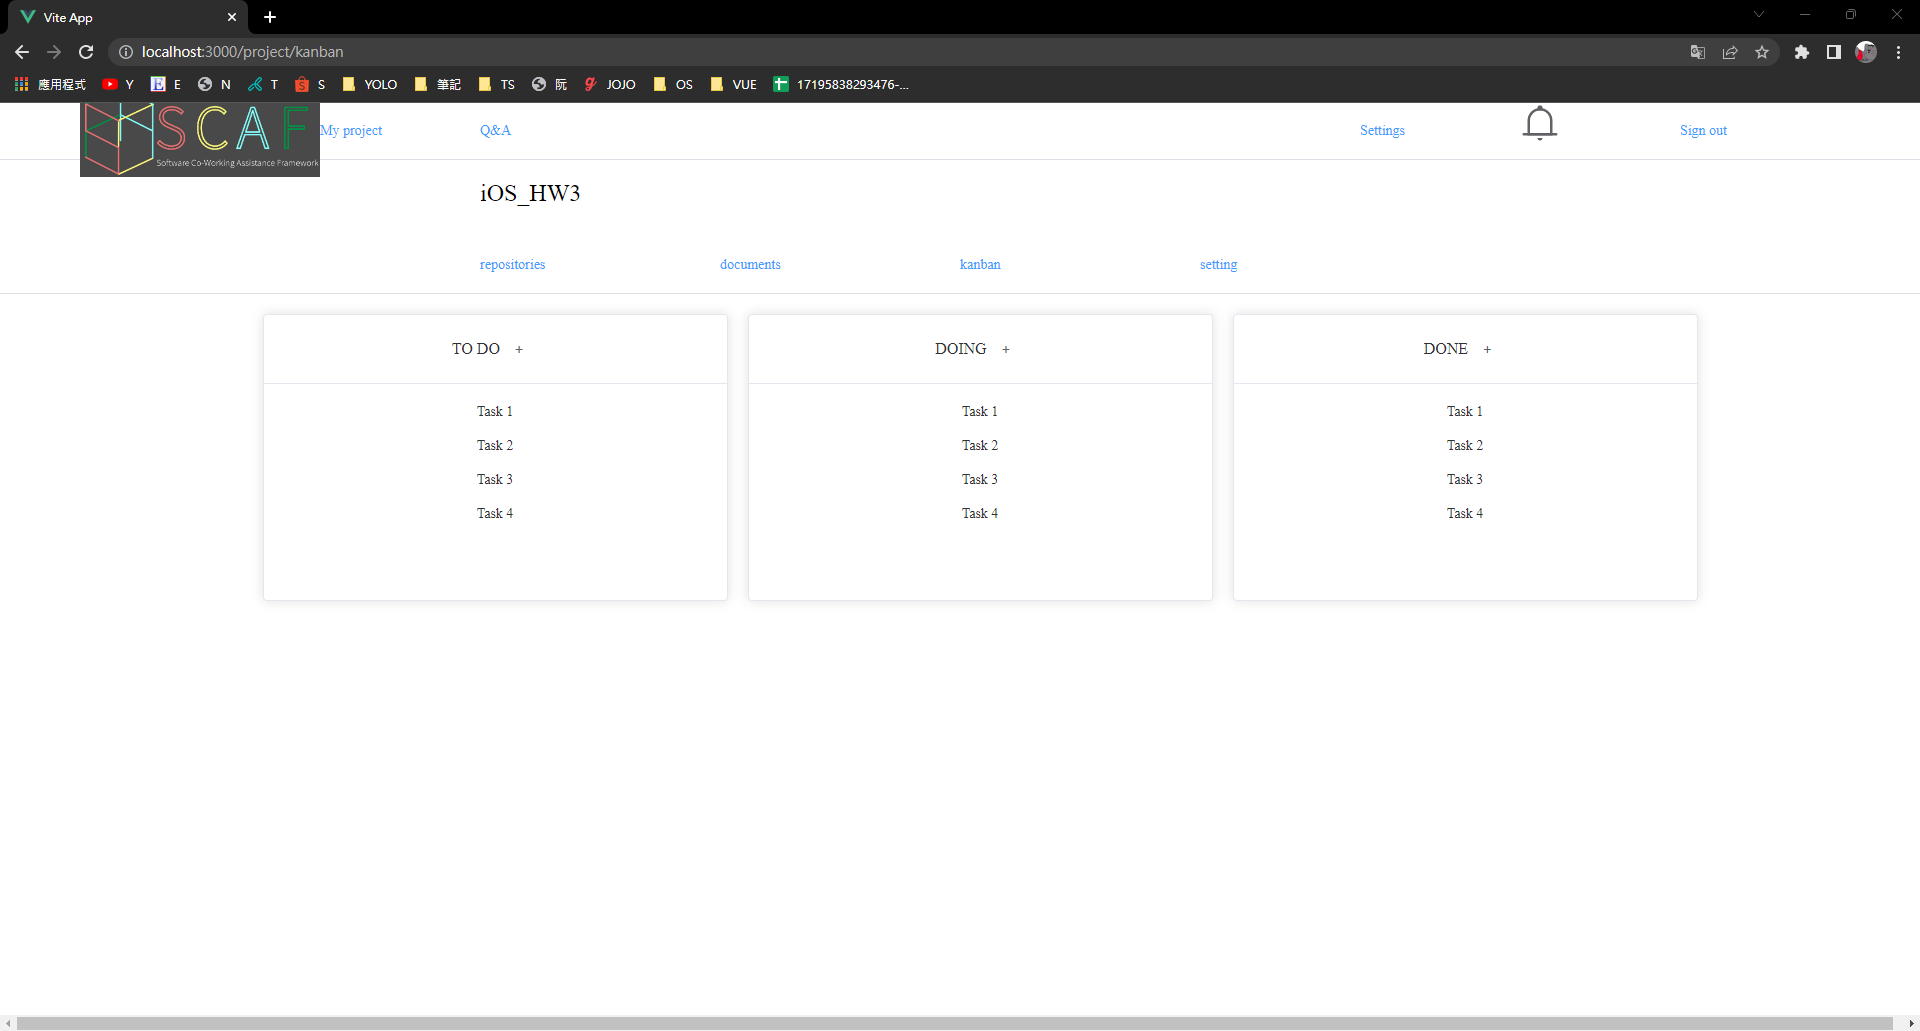
\includegraphics[width=0.9\textwidth]{assets/UI/kanban.png}
	\item 專案文件 \\ 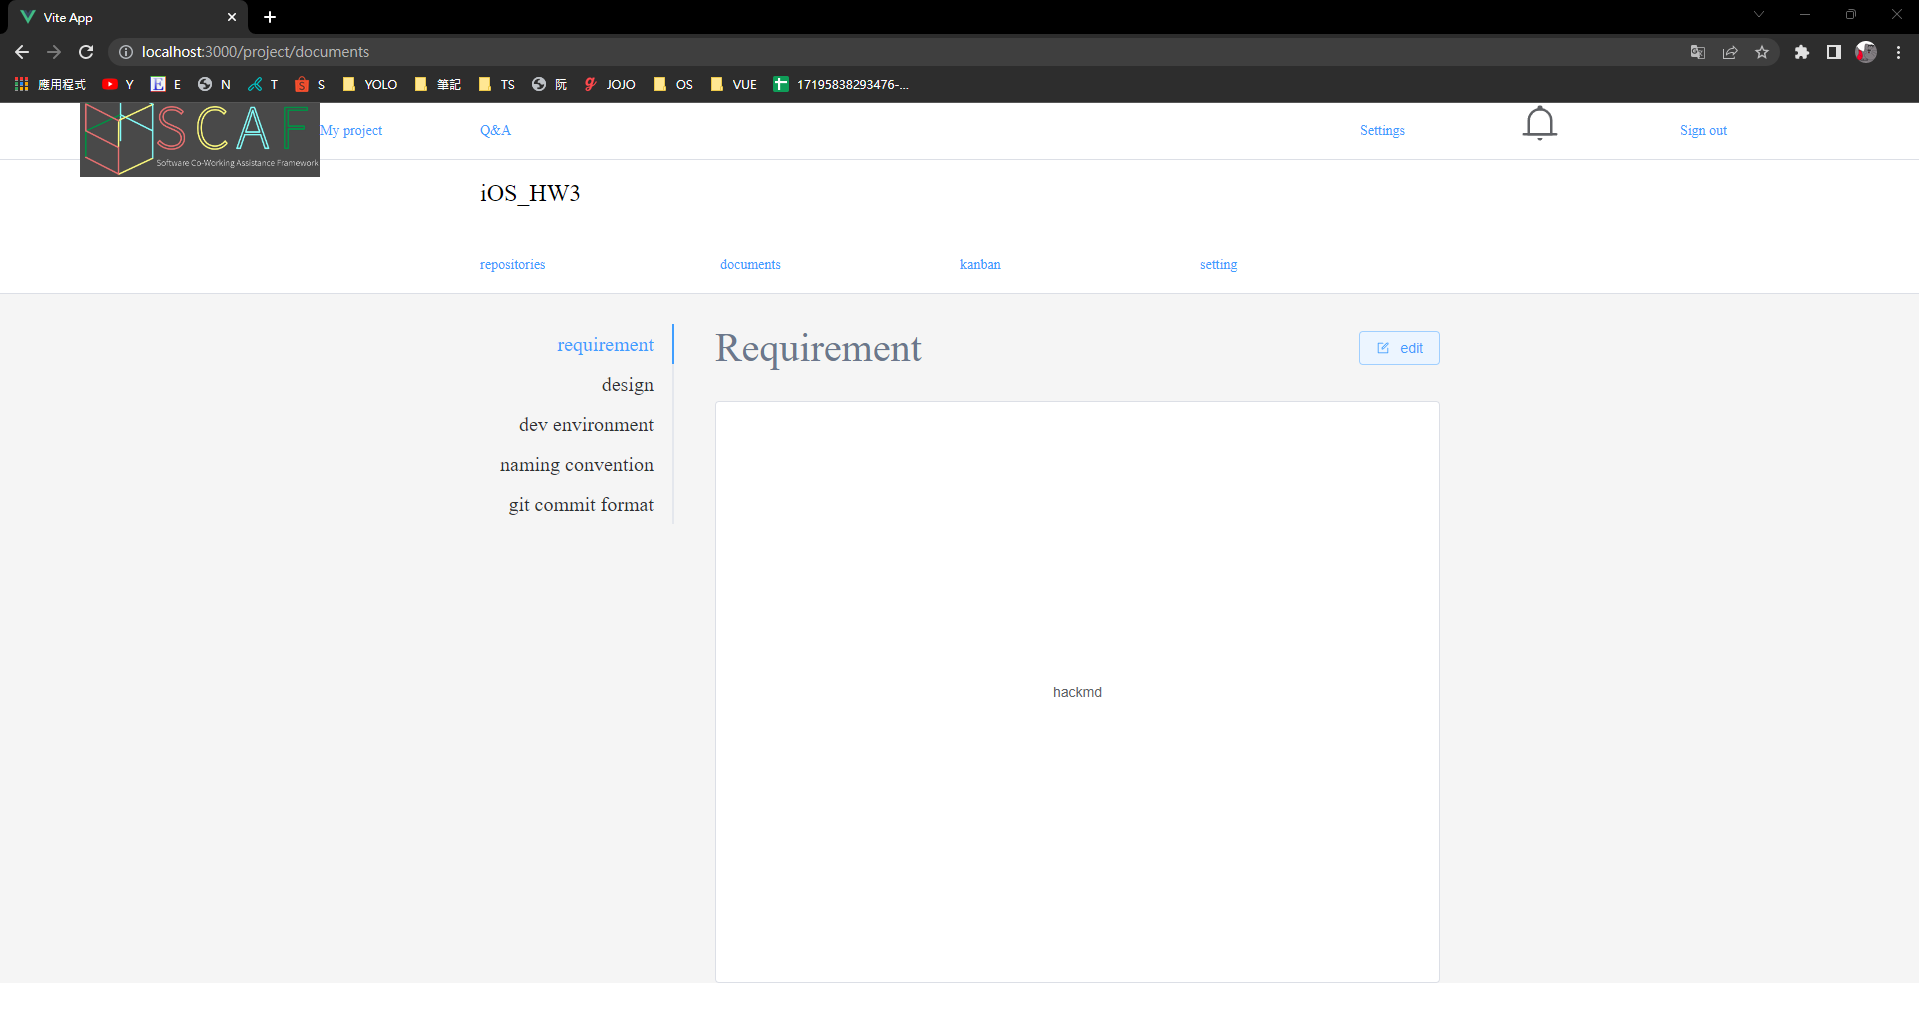
\includegraphics[width=0.9\textwidth]{assets/UI/doc.png}
	\item 刪除專案 \\ 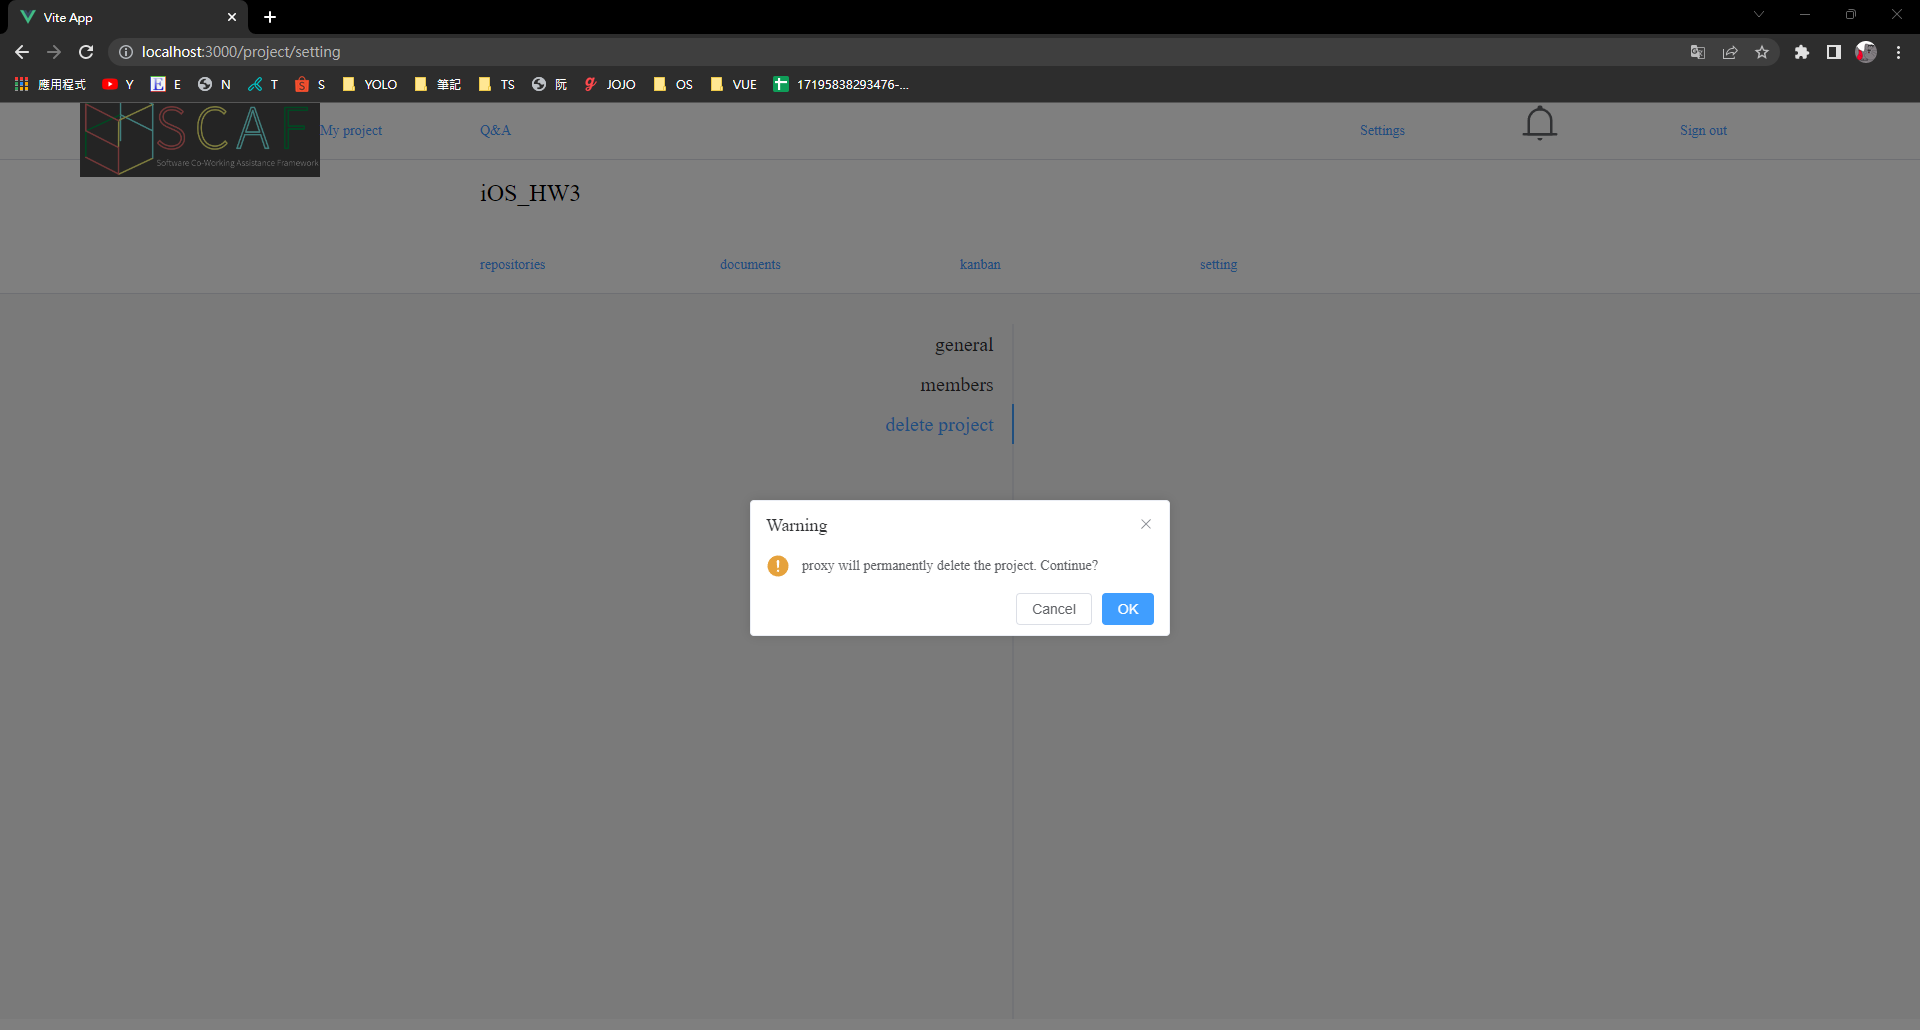
\includegraphics[width=0.9\textwidth]{assets/UI/delete_project.png}
	\item Q\&A \\ 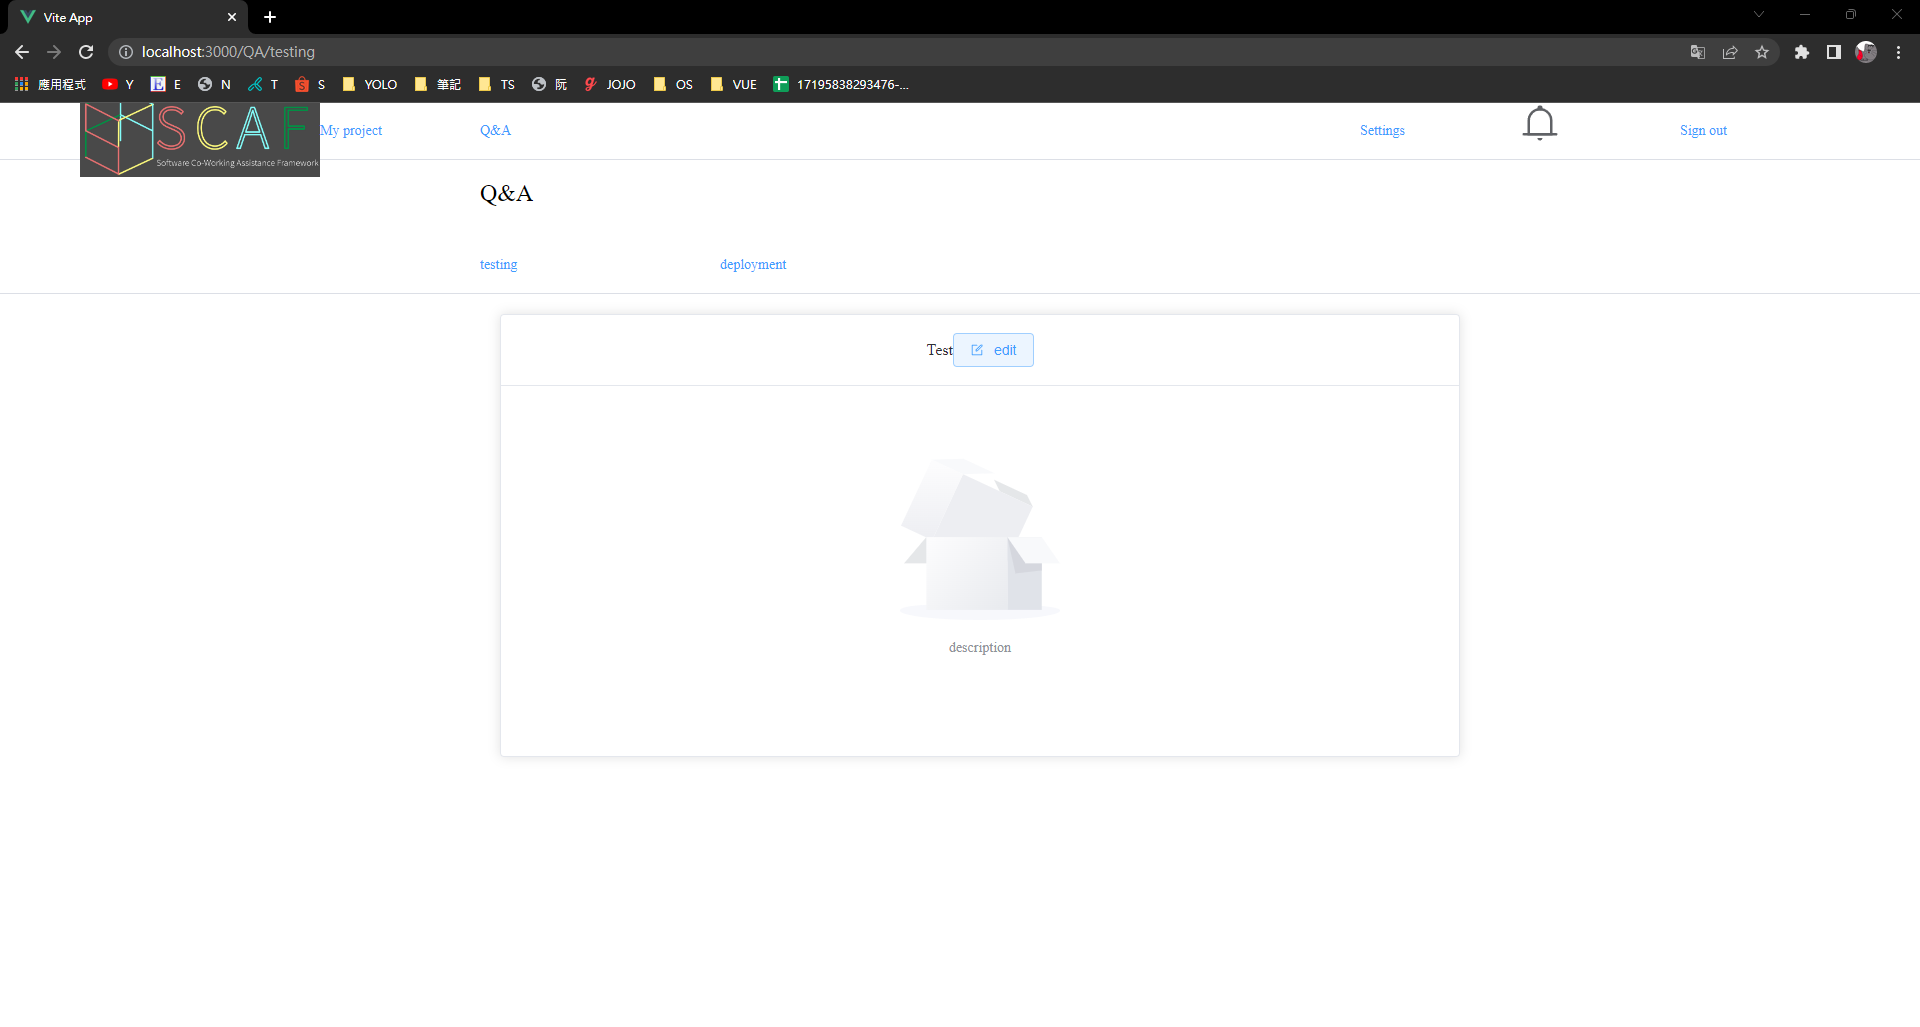
\includegraphics[width=0.9\textwidth]{assets/UI/QA.png}
\end{enumerate}

\section*{5. 資料設計(Data Design)}

% \begin{obeylines}
% 	\parindent=0pt
% 	設計此系統的資料庫schema、檔案結構、XML schema、JSON (JavaScript Object Notation)物件等。
% 	NoSQL 類似json格式
% 	簡
% \end{obeylines}

\begin{enumerate}
  \item User \\ \\
    \begin{tabular}{|l|l|l|l|}
      \hline
      \makecell[c]{欄位代碼} & \makecell[c]{欄位名稱} & \makecell[c]{欄位內容} & \makecell[c]{欄位型態} \\ \hline
      email & 電子郵件 & User的電子郵件 & string \\ \hline
      nikename & 姓名 & User的姓名 & string \\ \hline
      avatar & 大頭貼 & User的大頭貼 & string \\ \hline
      bio & 自我介紹 & User的自我介紹 & string \\ \hline
      projects & 專案 & User的全部專案ID & Array \\ \hline
    \end{tabular} \\
  \item Project \\ \\
    \begin{tabular}{|l|l|l|l|}
      \hline
      \makecell[c]{欄位代碼} & \makecell[c]{欄位名稱} & \makecell[c]{欄位內容} & \makecell[c]{欄位型態} \\ \hline
      id & 專案ID & 專案的ID & string \\ \hline
      name & 專案名稱 & 專案的名稱 & string \\ \hline
      members & 專案成員 & 專案的成員ID & Array<User> \\ \hline
      repositories & 專案repository & 專案的repositoryID & Array<Repo> \\ \hline
      documents & 專案文件 & 專案的文件ID & Array<Doc> \\ \hline
      tasks & 專案任務 & 專案的任務ID & Array<Tasks> \\ \hline
      dev\_tools & 專案開發工具 & 專案的開發工具ID & Array<string> \\ \hline
    \end{tabular} \\
  \item Repo \\ \\
    \begin{tabular}{|l|l|l|l|}
      \hline
      \makecell[c]{欄位代碼} & \makecell[c]{欄位名稱} & \makecell[c]{欄位內容} & \makecell[c]{欄位型態} \\ \hline
      id & repositoryID & repository的ID & string \\ \hline
      name & repository名稱 & repository的名稱 & string \\ \hline
      description & repository描述 & repository的描述 & string \\ \hline
      url & repository url & repository的url & Array<string> \\ \hline
    \end{tabular} \\
  \item Doc \\ \\ 
    \begin{tabular}{|l|l|l|l|}
      \hline
      \makecell[c]{欄位代碼} & \makecell[c]{欄位名稱} & \makecell[c]{欄位內容} & \makecell[c]{欄位型態} \\ \hline
      id & 文件ID & 文件的ID & string \\ \hline
      name & 文件名稱 & 文件的名稱 & string \\ \hline
      content & 文件內容 & 文件的內容 & string \\ \hline
    \end{tabular} \\
  \item Tasks \\ \\
    \begin{tabular}{|l|l|l|l|}
      \hline
      \makecell[c]{欄位代碼} & \makecell[c]{欄位名稱} & \makecell[c]{欄位內容} & \makecell[c]{欄位型態} \\ \hline
      id & 任務ID & 任務的ID & string \\ \hline
      name & 任務名稱 & 任務的名稱 & string \\ \hline
      description & 任務描述 & 任務的描述 & string \\ \hline
      status & 任務狀態 & 任務的狀態 & string \\ \hline
      deadline & 任務截止日期 & 任務的截止日期 & string \\ \hline
      assignee & 任務指派人 & 任務的指派人ID & User \\ \hline
      % comments & 任務討論 & 任務的討論ID & Array<Comment> \\ \hline
    \end{tabular} \\
  \item .scaf folder \\ \\
    \begin{tabular}{|l|l|l|l|}
      \hline
      \makecell[c]{欄位代碼} & \makecell[c]{欄位名稱} & \makecell[c]{欄位內容} & \makecell[c]{欄位型態} \\ \hline
    \end{tabular} \\
\end{enumerate}

\section*{6. 類別圖設計(Class Diagram)}

% \begin{obeylines}
% 	\parindent=0pt
% 	發展UML之class diagram (可對應C4 model中的Code diagram),明確設計系統中包含哪些類別,以及這些類別之間的關係。
% 	若遇到非一般物件類別或特殊物件類別,如HTML、JavaScript、JSP、Servlet等,可用stereotype表達,如<<JavaScript>>、<<Servlet>>。
% 	可把重點放在定義程式結構:訂出所有類別名稱、拉出所有類別關係,再加入重要的attibute/operation即可。而特殊的類別職責設計可加上文字說明。
% 	StarUML
% 	前後端都要
% \end{obeylines}

\section*{7. 實作方案(Implementation Languages and Platforms)}

% \begin{obeylines}
% 	\parindent=0pt
% 	說明系統之平台(如網站或行動App)
% 	說明預計採用的程式語言或技術(如後端Java、node.js、PHP等,前端JS+Boostrap、Android、iOS等)
% 	說明預計採用的框架(Framework,如前端React、Angular、Vue,後端Spring、SpringBoot等)、函式庫(如前端jQuery、d3.js,後端jsoup、iText)、Servless服務(Firebase)等。
% 	輕輕鬆酥
% \end{obeylines}
\begin{center}
	\begin{tabular}{|l|l|l|}
		\hline
		平台 & 網站 & CLI \\ \hline
		前端 & JavaScript & Go \\ \hline
		後端 & Go & Go \\ \hline
		前端框架 & Vue & Cobra \\ \hline	
		後端框架 & Gin & Gin \\ \hline
		資料庫 & Firebase & Firebase \\ \hline
		前後端溝通方式 & RESTful API & RESTful API \\ \hline
	\end{tabular}
\end{center}

\section*{8. 設計議題(Design Issue)}

\begin{enumerate}
	\item Golang沒有Firebase的客戶端SDK,無法使用Firebase。
	  \begin{enumerate}
			\item 解決方案
				\begin{enumerate}
					\item 自己寫一個library
					\item 將後端改成node.js
				\end{enumerate}
			\item 最後解決方案: 自己寫一個library
			\item 理由: 換另一個後端寫成本太高。
		\end{enumerate}
	\item 前端網頁的UI使用html手刻太過於花時間。
		\begin{enumerate}
			\item 解決方案
				\begin{enumerate}
					\item 慢慢刻到底
					\item 使用element-ui
				\end{enumerate}
			\item 最後解決方案: 使用element-ui
			\item 理由: 使用element-ui,可以減少開發時間,並且可以配合Vue。
		\end{enumerate}
	\item 在本地端的一個專案應該用什麼方式呈現?
		\begin{enumerate}
			\item 解決方案
				\begin{enumerate}
					\item 用一個檔案存所有資料
					\item 用一個資料夾存所有資料
					\item 直接讀取遠端的資料
				\end{enumerate}
			\item 最後解決方案: 用一個資料夾存一個專案的所有資料
			\item 理由
				\begin{enumerate}
					\item 讓本機即使是離線狀態也能使用
					\item 使用類似 git 的方式來管理專案
				\item 方便使用者控制專案的檔案
				\end{enumerate}
		\end{enumerate}
		\item 在本地端使用 SCAF 時,需要與遠端同步,應該使用什麼策略?
			\begin{enumerate}
				\item 可能解決方案:
					\begin{enumerate}
						\item 使用 git 進行版本控制,並利用 git 的合併功能,將本地端與遠端同步。
						\item 使用類似 google 文件的方式,版本只會是線性的,以最新修改的版本為主。但會有不同本地端的版本衝突的問題。
					\end{enumerate}
				\item 最後解決方案: 使用者執行同步指令時,將遠端與本地端強制更新成其中的最新版本,並儲存先前的版本成為一個快照。
				\item 理由:
					\begin{enumerate}
						\item 實作簡單
						\item 雖然無法合併不同版本,但能解決版本衝突問題
						\item 未來可以再加入合併功能
					\end{enumerate}	
			\end{enumerate}		
			\item 在 CLI 工具中新建專案時,會有必要與非必要設定(如名稱與開發流程),每個設定使用者都必須輸入一次選項,怎麼讓使用者的體驗更好?
			\begin{enumerate}
				\item 可能解決方案:
					\begin{enumerate}
					\item 使用者在新建專案時,只會有必要設定,非必要設定可以在專案建立後再設定。
					\item 使用者在新建專案時,需要輸入所有設定,包含必要與非必要設定。
					\end{enumerate}
				\item 最後解決方案:
				使用者在新建專案時,若使用 --default 參數,則只會有必要設定,非必要設定會設定為預設值,建立完成再去個別設定。
				若沒有使用 --default 參數,則需要輸入所有設定,但也可以在輸入時指定為預設值。
				\item 理由:
					\begin{enumerate}
						\item 使用者有彈性,可以選擇是否要使用預設值。
						\item 能讓使用者知道有哪些設定可以調整。
					\end{enumerate}
			\end{enumerate}
			\item 在 CLI 工具中,是否要使用指令來編輯 README 檔案?
				\begin{enumerate}
					\item 可能解決方案:
						\begin{enumerate}
							\item 使用指令編輯 README 檔案。
							\item 使用編輯器編輯 README 檔案。
						\end{enumerate}
					\item 最後解決方案: 使用編輯器直接編輯 README 檔案。
					\item 理由:
						\begin{enumerate}
							\item 使用者可以用自己習慣的編輯器。
							\item 使用者不會被指令綁住,較為彈性。
							\item 減少指令的複雜度。
						\end{enumerate}
				\end{enumerate}
			\item 在 CLI 工具中,專案開發工具(如 Kanban)的啟用要當作一般設定,或是獨立成一個子指令?
				\begin{enumerate}
					\item 可能解決方案:
						\begin{enumerate}
							\item 獨立成一個子指令。
							\item 將啟用作為一般設定。
						\end{enumerate}
					\item 最後解決方案: 將啟用作為一般設定。
					\item 理由:
						\begin{enumerate}
							\item 好讓使用者直接看到可以調整的設定。
							\item 減少指令的複雜度。
							\item 提高操作頻率,使用者可以更容易地啟用/停用開發工具。
						\end{enumerate}
				\end{enumerate}
			\item 在 CLI 工具中,是否要支援讓使用者自訂指令?
				\begin{enumerate}
					\item 可能解決方案:
						\begin{enumerate}
							\item 支援讓使用者自訂指令。
							\item 不支援讓使用者自訂指令。
						\end{enumerate}
					\item 最後解決方案: 支援讓使用者自訂指令。
					\item 理由:
						\begin{enumerate}
							\item 增加使用者的彈性,使用者可以根據自己的喜好和需求自行設計指令。
							\item 提高使用者的滿意度,使用者能夠運用更多的功能。
							\item 有助於指令的擴充,讓 CLI 工具更完整。
						\end{enumerate}
				\end{enumerate}
			\item API 網址設計,parameter 的請求方式。
				\begin{enumerate}
					\item 可能解決方案:
						\begin{enumerate}
							\item 使用 query string。
							\item 使用 path parameter。
						\end{enumerate}
					\item 最後解決方案: 使用 path parameter。
					\item 理由:
						\begin{enumerate}
							\item 使用者可以直接在網址中看到參數。
							\item 減少使用者的複雜度。
							\item 減少使用者的輸入量。
						\end{enumerate}
				\end{enumerate}
\end{enumerate}

\end{document}